%\pdfoutput=1
% Uncomment line above if submitting to arXiv and using pdflatex

% $Id: main.tex 33041 2013-03-25 16:12:53Z tgershon $
% ============================================================================
% Purpose: Template for LHCb documents
% Authors: Tomasz Skwarnicki, Roger Forty, Ulrik Egede
% Modified by: Adam Elwood
% Created on: 2010-09-24
% ============================================================================
\documentclass[12pt,a4paper]{article}
% For two column text, add "twocolumn" as an option to the document
% class. Also uncomment the two "onecolumn" and "twocolumn" lines
% around the title page below.

% Variables that controls behaviour
\usepackage{ifthen} % for conditional statements
\newboolean{pdflatex}
\setboolean{pdflatex}{true} % False for eps figures 

\newboolean{articletitles}
\setboolean{articletitles}{true} % False removes titles in references

\newboolean{uprightparticles}
\setboolean{uprightparticles}{false} %True for upright particle symbols

%\newboolean{inbibliography}
%\setboolean{inbibliography}{false} %True once you enter the bibliography

% THis file contains all the default packages and modifications for
% LHCb formatting

%% %%%%%%%%%%%%%%%%%%
%%  Page formatting
%% %%%%%%%%%%%%%%%%%%
\textheight=230mm
\textwidth=160mm
\oddsidemargin=7mm
\evensidemargin=-10mm
\topmargin=-10mm
\headsep=20mm
\columnsep=5mm
\addtolength{\belowcaptionskip}{0.5em}

\renewcommand{\textfraction}{0.01}
\renewcommand{\floatpagefraction}{0.99}
\renewcommand{\topfraction}{0.9}
\renewcommand{\bottomfraction}{0.9}


\setlength{\hoffset}{-2cm}
\setlength{\voffset}{-2cm}
% Page defaults ...
\topmargin=0.5cm
\oddsidemargin=2.5cm
\textwidth=16cm
\textheight=22cm
% Allow the page size to vary a bit ...
\raggedbottom
% To avoid Latex to be too fussy with line breaking ...
%\sloppy

%% %%%%%%%%%%%%%%%%%%%%%%%
%% Packages to be used
%% %%%%%%%%%%%%%%%%%%%%%%% 
\usepackage{microtype}
\usepackage{lineno}  % for line numbering during review
\usepackage{xspace} % To avoid problems with missing or double spaces after
                    % predefined symbold
\usepackage{caption} %these three command get the figure and table captions automatically small
\renewcommand{\captionfont}{\small}
\renewcommand{\captionlabelfont}{\small}

%% Graphics
\usepackage{graphicx}  % to include figures (can also use other packages)
\usepackage{color}
\usepackage{colortbl}
\graphicspath{{./figs/}} % Make Latex search fig subdir for figures
\usepackage{cancel}
\usepackage{subfigure}

%% Math
\usepackage{amsmath} % Adds a large collection of math symbols
\usepackage{amssymb}
\usepackage{amsfonts}
\usepackage{upgreek} % Adds in support for greek letters in roman typeset

%% fix to allow peaceful coexistence of line numbering and
%% mathematical objects
%% http://www.latex-community.org/forum/viewtopic.php?f=5&t=163
%%
\newcommand*\patchAmsMathEnvironmentForLineno[1]{%
\expandafter\let\csname old#1\expandafter\endcsname\csname #1\endcsname
\expandafter\let\csname oldend#1\expandafter\endcsname\csname
end#1\endcsname
 \renewenvironment{#1}%
   {\linenomath\csname old#1\endcsname}%
   {\csname oldend#1\endcsname\endlinenomath}%
}
\newcommand*\patchBothAmsMathEnvironmentsForLineno[1]{%
  \patchAmsMathEnvironmentForLineno{#1}%
  \patchAmsMathEnvironmentForLineno{#1*}%
}
\AtBeginDocument{%
\patchBothAmsMathEnvironmentsForLineno{equation}%
\patchBothAmsMathEnvironmentsForLineno{align}%
\patchBothAmsMathEnvironmentsForLineno{flalign}%
\patchBothAmsMathEnvironmentsForLineno{alignat}%
\patchBothAmsMathEnvironmentsForLineno{gather}%
\patchBothAmsMathEnvironmentsForLineno{multline}%
}

% Get hyperlinks to captions and in references.
% These do not work with revtex. Use "hypertext" as class option instead.
\usepackage{hyperref}    % Hyperlinks in references
\usepackage[all]{hypcap} % Internal hyperlinks to floats.

%%% $Id: lhcb-symbols-def.tex 39235 2013-07-16 11:13:01Z roldeman $
%%% ======================================================================
%%% Purpose: Standard LHCb aliases
%%% Author: Originally Ulrik Egede, adapted by Tomasz Skwarnicki for templates,
%%% rewritten by Chris Parkes
%%% Maintainer : Ulrik Egede (2010 - 2012)
%%% =======================================================================

%%% To use this file outside the normal LHCb document environment, the
%%% following should be added in a preamble (before \begin{document}
%%%
%%%\usepackage{ifthen} 
%%%\newboolean{uprightparticles}
%%%\setboolean{uprightparticles}{false} %Set true for upright particle symbols
%%% \usepackage{xspace} 
%%% \usepackage{upgreek}

%%%%%%%%%%%%%%%%%%%%%%%%%%%%%%%%%%%%%%%%%%%%%%%%%%%%%%%%%%%%
%%%
%%% The following is to ensure that the template automatically can process
%%% this file.
%%%
%%% Add comments with at least three %%% preceding.
%%% Add new sections with one % preceding
%%% Add new subsections with two %% preceding
%%%%%%%%%%%%%%%%%%%%%%%%%%%%%%%%%%%%%%%%%%%%%%%%%%%%%%%%%%%%

%%%%%%%%%%%%%
% Experiments
%%%%%%%%%%%%%
\def\lhcb {\mbox{LHCb}\xspace}
\def\atlas  {\mbox{ATLAS}\xspace}
\def\cms    {\mbox{CMS}\xspace}
\def\alice  {\mbox{ALICE}\xspace}
\def\babar  {\mbox{BaBar}\xspace}
\def\belle  {\mbox{Belle}\xspace}
\def\cleo   {\mbox{CLEO}\xspace}
\def\cdf    {\mbox{CDF}\xspace}
\def\dzero  {\mbox{D0}\xspace}
\def\aleph  {\mbox{ALEPH}\xspace}
\def\delphi {\mbox{DELPHI}\xspace}
\def\opal   {\mbox{OPAL}\xspace}
\def\lthree {\mbox{L3}\xspace}
\def\sld    {\mbox{SLD}\xspace}
%%%\def\argus  {\mbox{ARGUS}\xspace}
%%%\def\uaone  {\mbox{UA1}\xspace}
%%%\def\uatwo  {\mbox{UA2}\xspace}
%%%\def\ux85 {\mbox{UX85}\xspace}
\def\cern {\mbox{CERN}\xspace}
\def\lhc    {\mbox{LHC}\xspace}
\def\lep    {\mbox{LEP}\xspace}
\def\tevatron {Tevatron\xspace}

%% LHCb sub-detectors and sub-systems

%%%\def\pu     {PU\xspace}
\def\velo   {VELO\xspace}
\def\rich   {RICH\xspace}
\def\richone {RICH1\xspace}
\def\richtwo {RICH2\xspace}
\def\ttracker {TT\xspace}
\def\intr   {IT\xspace}
\def\st     {ST\xspace}
\def\ot     {OT\xspace}
%%%\def\Tone   {T1\xspace}
%%%\def\Ttwo   {T2\xspace}
%%%\def\Tthree {T3\xspace}
%%%\def\Mone   {M1\xspace}
%%%\def\Mtwo   {M2\xspace}
%%%\def\Mthree {M3\xspace}
%%%\def\Mfour  {M4\xspace}
%%%\def\Mfive  {M5\xspace}
\def\spd    {SPD\xspace}
\def\presh  {PS\xspace}
\def\ecal   {ECAL\xspace}
\def\hcal   {HCAL\xspace}
%%%\def\bcm    {BCM\xspace}

%%%\def\ode    {ODE\xspace}
%%%\def\daq    {DAQ\xspace}
%%%\def\tfc    {TFC\xspace}
%%%\def\ecs    {ECS\xspace}
%%%\def\lone   {L0\xspace}
%%%\def\hlt    {HLT\xspace}
%%%\def\hltone {HLT1\xspace}
%%%\def\hlttwo {HLT2\xspace}

%%% Upright (not slanted) Particles

\ifthenelse{\boolean{uprightparticles}}%
{\def\Palpha      {\ensuremath{\upalpha}\xspace}
 \def\Pbeta       {\ensuremath{\upbeta}\xspace}
 \def\Pgamma      {\ensuremath{\upgamma}\xspace}                 
 \def\Pdelta      {\ensuremath{\updelta}\xspace}                 
 \def\Pepsilon    {\ensuremath{\upepsilon}\xspace}                 
 \def\Pvarepsilon {\ensuremath{\upvarepsilon}\xspace}                 
 \def\Pzeta       {\ensuremath{\upzeta}\xspace}                 
 \def\Peta        {\ensuremath{\upeta}\xspace}                 
 \def\Ptheta      {\ensuremath{\uptheta}\xspace}                 
 \def\Pvartheta   {\ensuremath{\upvartheta}\xspace}                 
 \def\Piota       {\ensuremath{\upiota}\xspace}                 
 \def\Pkappa      {\ensuremath{\upkappa}\xspace}                 
 \def\Plambda     {\ensuremath{\uplambda}\xspace}                 
 \def\Pmu         {\ensuremath{\upmu}\xspace}                 
 \def\Pnu         {\ensuremath{\upnu}\xspace}                 
 \def\Pxi         {\ensuremath{\upxi}\xspace}                 
 \def\Ppi         {\ensuremath{\uppi}\xspace}                 
 \def\Pvarpi      {\ensuremath{\upvarpi}\xspace}                 
 \def\Prho        {\ensuremath{\uprho}\xspace}                 
 \def\Pvarrho     {\ensuremath{\upvarrho}\xspace}                 
 \def\Ptau        {\ensuremath{\uptau}\xspace}                 
 \def\Pupsilon    {\ensuremath{\upupsilon}\xspace}                 
 \def\Pphi        {\ensuremath{\upphi}\xspace}                 
 \def\Pvarphi     {\ensuremath{\upvarphi}\xspace}                 
 \def\Pchi        {\ensuremath{\upchi}\xspace}                 
 \def\Ppsi        {\ensuremath{\uppsi}\xspace}                 
 \def\Pomega      {\ensuremath{\upomega}\xspace}                 

 \def\PDelta      {\ensuremath{\Delta}\xspace}                 
 \def\PXi      {\ensuremath{\Xi}\xspace}                 
 \def\PLambda      {\ensuremath{\Lambda}\xspace}                 
 \def\PSigma      {\ensuremath{\Sigma}\xspace}                 
 \def\POmega      {\ensuremath{\Omega}\xspace}                 
 \def\PUpsilon      {\ensuremath{\Upsilon}\xspace}                 
 
 %\mathchardef\Deltares="7101
 %\mathchardef\Xi="7104
 %\mathchardef\Lambda="7103
 %\mathchardef\Sigma="7106
 %\mathchardef\Omega="710A


 \def\PA      {\ensuremath{\mathrm{A}}\xspace}                 
 \def\PB      {\ensuremath{\mathrm{B}}\xspace}                 
 \def\PC      {\ensuremath{\mathrm{C}}\xspace}                 
 \def\PD      {\ensuremath{\mathrm{D}}\xspace}                 
 \def\PE      {\ensuremath{\mathrm{E}}\xspace}                 
 \def\PF      {\ensuremath{\mathrm{F}}\xspace}                 
 \def\PG      {\ensuremath{\mathrm{G}}\xspace}                 
 \def\PH      {\ensuremath{\mathrm{H}}\xspace}                 
 \def\PI      {\ensuremath{\mathrm{I}}\xspace}                 
 \def\PJ      {\ensuremath{\mathrm{J}}\xspace}                 
 \def\PK      {\ensuremath{\mathrm{K}}\xspace}                 
 \def\PL      {\ensuremath{\mathrm{L}}\xspace}                 
 \def\PM      {\ensuremath{\mathrm{M}}\xspace}                 
 \def\PN      {\ensuremath{\mathrm{N}}\xspace}                 
 \def\PO      {\ensuremath{\mathrm{O}}\xspace}                 
 \def\PP      {\ensuremath{\mathrm{P}}\xspace}                 
 \def\PQ      {\ensuremath{\mathrm{Q}}\xspace}                 
 \def\PR      {\ensuremath{\mathrm{R}}\xspace}                 
 \def\PS      {\ensuremath{\mathrm{S}}\xspace}                 
 \def\PT      {\ensuremath{\mathrm{T}}\xspace}                 
 \def\PU      {\ensuremath{\mathrm{U}}\xspace}                 
 \def\PV      {\ensuremath{\mathrm{V}}\xspace}                 
 \def\PW      {\ensuremath{\mathrm{W}}\xspace}                 
 \def\PX      {\ensuremath{\mathrm{X}}\xspace}                 
 \def\PY      {\ensuremath{\mathrm{Y}}\xspace}                 
 \def\PZ      {\ensuremath{\mathrm{Z}}\xspace}                 
 \def\Pa      {\ensuremath{\mathrm{a}}\xspace}                 
 \def\Pb      {\ensuremath{\mathrm{b}}\xspace}                 
 \def\Pc      {\ensuremath{\mathrm{c}}\xspace}                 
 \def\Pd      {\ensuremath{\mathrm{d}}\xspace}                 
 \def\Pe      {\ensuremath{\mathrm{e}}\xspace}                 
 \def\Pf      {\ensuremath{\mathrm{f}}\xspace}                 
 \def\Pg      {\ensuremath{\mathrm{g}}\xspace}                 
 \def\Ph      {\ensuremath{\mathrm{h}}\xspace}                 
 \def\Pi      {\ensuremath{\mathrm{i}}\xspace}                 
 \def\Pj      {\ensuremath{\mathrm{j}}\xspace}                 
 \def\Pk      {\ensuremath{\mathrm{k}}\xspace}                 
 \def\Pl      {\ensuremath{\mathrm{l}}\xspace}                 
 \def\Pm      {\ensuremath{\mathrm{m}}\xspace}                 
 \def\Pn      {\ensuremath{\mathrm{n}}\xspace}                 
 \def\Po      {\ensuremath{\mathrm{o}}\xspace}                 
 \def\Pp      {\ensuremath{\mathrm{p}}\xspace}                 
 \def\Pq      {\ensuremath{\mathrm{q}}\xspace}                 
 \def\Pr      {\ensuremath{\mathrm{r}}\xspace}                 
 \def\Ps      {\ensuremath{\mathrm{s}}\xspace}                 
 \def\Pt      {\ensuremath{\mathrm{t}}\xspace}                 
 \def\Pu      {\ensuremath{\mathrm{u}}\xspace}                 
 \def\Pv      {\ensuremath{\mathrm{v}}\xspace}                 
 \def\Pw      {\ensuremath{\mathrm{w}}\xspace}                 
 \def\Px      {\ensuremath{\mathrm{x}}\xspace}                 
 \def\Py      {\ensuremath{\mathrm{y}}\xspace}                 
 \def\Pz      {\ensuremath{\mathrm{z}}\xspace}                 
}
{\def\Palpha      {\ensuremath{\alpha}\xspace}
 \def\Pbeta       {\ensuremath{\beta}\xspace}
 \def\Pgamma      {\ensuremath{\gamma}\xspace}                 
 \def\Pdelta      {\ensuremath{\delta}\xspace}                 
 \def\Pepsilon    {\ensuremath{\epsilon}\xspace}                 
 \def\Pvarepsilon {\ensuremath{\varepsilon}\xspace}                 
 \def\Pzeta       {\ensuremath{\zeta}\xspace}                 
 \def\Peta        {\ensuremath{\eta}\xspace}                 
 \def\Ptheta      {\ensuremath{\theta}\xspace}                 
 \def\Pvartheta   {\ensuremath{\vartheta}\xspace}                 
 \def\Piota       {\ensuremath{\iota}\xspace}                 
 \def\Pkappa      {\ensuremath{\kappa}\xspace}                 
 \def\Plambda     {\ensuremath{\lambda}\xspace}                 
 \def\Pmu         {\ensuremath{\mu}\xspace}                 
 \def\Pnu         {\ensuremath{\nu}\xspace}                 
 \def\Pxi         {\ensuremath{\xi}\xspace}                 
 \def\Ppi         {\ensuremath{\pi}\xspace}                 
 \def\Pvarpi      {\ensuremath{\varpi}\xspace}                 
 \def\Prho        {\ensuremath{\rho}\xspace}                 
 \def\Pvarrho     {\ensuremath{\varrho}\xspace}                 
 \def\Ptau        {\ensuremath{\tau}\xspace}                 
 \def\Pupsilon    {\ensuremath{\upsilon}\xspace}                 
 \def\Pphi        {\ensuremath{\phi}\xspace}                 
 \def\Pvarphi     {\ensuremath{\varphi}\xspace}                 
 \def\Pchi        {\ensuremath{\chi}\xspace}                 
 \def\Ppsi        {\ensuremath{\psi}\xspace}                 
 \def\Pomega      {\ensuremath{\omega}\xspace}                 
 \mathchardef\PDelta="7101
 \mathchardef\PXi="7104
 \mathchardef\PLambda="7103
 \mathchardef\PSigma="7106
 \mathchardef\POmega="710A
 \mathchardef\PUpsilon="7107
 \def\PA      {\ensuremath{A}\xspace}                 
 \def\PB      {\ensuremath{B}\xspace}                 
 \def\PC      {\ensuremath{C}\xspace}                 
 \def\PD      {\ensuremath{D}\xspace}                 
 \def\PE      {\ensuremath{E}\xspace}                 
 \def\PF      {\ensuremath{F}\xspace}                 
 \def\PG      {\ensuremath{G}\xspace}                 
 \def\PH      {\ensuremath{H}\xspace}                 
 \def\PI      {\ensuremath{I}\xspace}                 
 \def\PJ      {\ensuremath{J}\xspace}                 
 \def\PK      {\ensuremath{K}\xspace}                 
 \def\PL      {\ensuremath{L}\xspace}                 
 \def\PM      {\ensuremath{M}\xspace}                 
 \def\PN      {\ensuremath{N}\xspace}                 
 \def\PO      {\ensuremath{O}\xspace}                 
 \def\PP      {\ensuremath{P}\xspace}                 
 \def\PQ      {\ensuremath{Q}\xspace}                 
 \def\PR      {\ensuremath{R}\xspace}                 
 \def\PS      {\ensuremath{S}\xspace}                 
 \def\PT      {\ensuremath{T}\xspace}                 
 \def\PU      {\ensuremath{U}\xspace}                 
 \def\PV      {\ensuremath{V}\xspace}                 
 \def\PW      {\ensuremath{W}\xspace}                 
 \def\PX      {\ensuremath{X}\xspace}                 
 \def\PY      {\ensuremath{Y}\xspace}                 
 \def\PZ      {\ensuremath{Z}\xspace}                 
 \def\Pa      {\ensuremath{a}\xspace}                 
 \def\Pb      {\ensuremath{b}\xspace}                 
 \def\Pc      {\ensuremath{c}\xspace}                 
 \def\Pd      {\ensuremath{d}\xspace}                 
 \def\Pe      {\ensuremath{e}\xspace}                 
 \def\Pf      {\ensuremath{f}\xspace}                 
 \def\Pg      {\ensuremath{g}\xspace}                 
 \def\Ph      {\ensuremath{h}\xspace}                 
 \def\Pi      {\ensuremath{i}\xspace}                 
 \def\Pj      {\ensuremath{j}\xspace}                 
 \def\Pk      {\ensuremath{k}\xspace}                 
 \def\Pl      {\ensuremath{l}\xspace}                 
 \def\Pm      {\ensuremath{m}\xspace}                 
 \def\Pn      {\ensuremath{n}\xspace}                 
 \def\Po      {\ensuremath{o}\xspace}                 
 \def\Pp      {\ensuremath{p}\xspace}                 
 \def\Pq      {\ensuremath{q}\xspace}                 
 \def\Pr      {\ensuremath{r}\xspace}                 
 \def\Ps      {\ensuremath{s}\xspace}                 
 \def\Pt      {\ensuremath{t}\xspace}                 
 \def\Pu      {\ensuremath{u}\xspace}                 
 \def\Pv      {\ensuremath{v}\xspace}                 
 \def\Pw      {\ensuremath{w}\xspace}                 
 \def\Px      {\ensuremath{x}\xspace}                 
 \def\Py      {\ensuremath{y}\xspace}                 
 \def\Pz      {\ensuremath{z}\xspace}                 
}

%%%%%%%%%%%%%%%%%%%%%%%%%%%%%%%%%%%%%%%%%%%%%%%
% Particles

%% Leptons

\let\emi\en
\def\electron   {\ensuremath{\Pe}\xspace}
\def\en         {\ensuremath{\Pe^-}\xspace}   % electron negative (\em is taken)
\def\ep         {\ensuremath{\Pe^+}\xspace}
\def\epm        {\ensuremath{\Pe^\pm}\xspace} 
\def\epem       {\ensuremath{\Pe^+\Pe^-}\xspace}
%%%\def\ee         {\ensuremath{\Pe^-\Pe^-}\xspace}

\def\mmu        {\ensuremath{\Pmu}\xspace}
\def\mup        {\ensuremath{\Pmu^+}\xspace}
\def\mun        {\ensuremath{\Pmu^-}\xspace} % muon negative (\mum is taken)
\def\mumu       {\ensuremath{\Pmu^+\Pmu^-}\xspace}
\def\mtau       {\ensuremath{\Ptau}\xspace}

\def\taup       {\ensuremath{\Ptau^+}\xspace}
\def\taum       {\ensuremath{\Ptau^-}\xspace}
\def\tautau     {\ensuremath{\Ptau^+\Ptau^-}\xspace}

\def\ellm       {\ensuremath{\ell^-}\xspace}
\def\ellp       {\ensuremath{\ell^+}\xspace}
%%%\def\ellell     {\ensuremath{\ell^+ \ell^-}\xspace}

\def\neu        {\ensuremath{\Pnu}\xspace}
\def\neub       {\ensuremath{\overline{\Pnu}}\xspace}
%%%\def\nuenueb    {\ensuremath{\neu\neub}\xspace}
\def\neue       {\ensuremath{\neu_e}\xspace}
\def\neueb      {\ensuremath{\neub_e}\xspace}
%%%\def\neueneueb  {\ensuremath{\neue\neueb}\xspace}
\def\neum       {\ensuremath{\neu_\mu}\xspace}
\def\neumb      {\ensuremath{\neub_\mu}\xspace}
%%%\def\neumneumb  {\ensuremath{\neum\neumb}\xspace}
\def\neut       {\ensuremath{\neu_\tau}\xspace}
\def\neutb      {\ensuremath{\neub_\tau}\xspace}
%%%\def\neutneutb  {\ensuremath{\neut\neutb}\xspace}
\def\neul       {\ensuremath{\neu_\ell}\xspace}
\def\neulb      {\ensuremath{\neub_\ell}\xspace}
%%%\def\neulneulb  {\ensuremath{\neul\neulb}\xspace}

%% Gauge bosons and scalars

\def\g      {\ensuremath{\Pgamma}\xspace}
\def\H      {\ensuremath{\PH^0}\xspace}
\def\Hp     {\ensuremath{\PH^+}\xspace}
\def\Hm     {\ensuremath{\PH^-}\xspace}
\def\Hpm    {\ensuremath{\PH^\pm}\xspace}
\def\W      {\ensuremath{\PW}\xspace}
\def\Wp     {\ensuremath{\PW^+}\xspace}
\def\Wm     {\ensuremath{\PW^-}\xspace}
\def\Wpm    {\ensuremath{\PW^\pm}\xspace}
\def\Z      {\ensuremath{\PZ}\xspace}

%% Quarks

\def\quark     {\ensuremath{\Pq}\xspace}
\def\quarkbar  {\ensuremath{\overline \quark}\xspace}
\def\qqbar     {\ensuremath{\quark\quarkbar}\xspace}
\def\uquark    {\ensuremath{\Pu}\xspace}
\def\uquarkbar {\ensuremath{\overline \uquark}\xspace}
\def\uubar     {\ensuremath{\uquark\uquarkbar}\xspace}
\def\dquark    {\ensuremath{\Pd}\xspace}
\def\dquarkbar {\ensuremath{\overline \dquark}\xspace}
\def\ddbar     {\ensuremath{\dquark\dquarkbar}\xspace}
\def\squark    {\ensuremath{\Ps}\xspace}
\def\squarkbar {\ensuremath{\overline \squark}\xspace}
\def\ssbar     {\ensuremath{\squark\squarkbar}\xspace}
\def\cquark    {\ensuremath{\Pc}\xspace}
\def\cquarkbar {\ensuremath{\overline \cquark}\xspace}
\def\ccbar     {\ensuremath{\cquark\cquarkbar}\xspace}
\def\bquark    {\ensuremath{\Pb}\xspace}
\def\bquarkbar {\ensuremath{\overline \bquark}\xspace}
\def\bbbar     {\ensuremath{\bquark\bquarkbar}\xspace}
\def\tquark    {\ensuremath{\Pt}\xspace}
\def\tquarkbar {\ensuremath{\overline \tquark}\xspace}
\def\ttbar     {\ensuremath{\tquark\tquarkbar}\xspace}

%% Light mesons

\def\pion  {\ensuremath{\Ppi}\xspace}
\def\piz   {\ensuremath{\pion^0}\xspace}
\def\pizs  {\ensuremath{\pion^0\mbox\,\rm{s}}\xspace}
%%%\def\ppz   {\ensuremath{\pion^0\pion^0}\xspace}
\def\pip   {\ensuremath{\pion^+}\xspace}
\def\pim   {\ensuremath{\pion^-}\xspace}
%%%\def\pipi  {\ensuremath{\pion^+\pion^-}\xspace}
\def\pipm  {\ensuremath{\pion^\pm}\xspace}
\def\pimp  {\ensuremath{\pion^\mp}\xspace}

\def\kaon  {\ensuremath{\PK}\xspace}
%%% do NOT use ensuremath here
  \def\Kbar  {\kern 0.2em\overline{\kern -0.2em \PK}{}\xspace}
\def\Kb    {\ensuremath{\Kbar}\xspace}
\def\Kz    {\ensuremath{\kaon^0}\xspace}
\def\Kzb   {\ensuremath{\Kbar^0}\xspace}
%%%\def\KzKzb {\ensuremath{\Kz \kern -0.16em \Kzb}\xspace}
\def\Kp    {\ensuremath{\kaon^+}\xspace}
\def\Km    {\ensuremath{\kaon^-}\xspace}
\def\Kpm   {\ensuremath{\kaon^\pm}\xspace}
\def\Kmp   {\ensuremath{\kaon^\mp}\xspace}
%%%\def\KpKm  {\ensuremath{\Kp \kern -0.16em \Km}\xspace}
\def\KS    {\ensuremath{\kaon^0_{\rm\scriptscriptstyle S}}\xspace} 
\def\KL    {\ensuremath{\kaon^0_{\rm\scriptscriptstyle L}}\xspace} 
\def\Kstarz  {\ensuremath{\kaon^{*0}}\xspace}
\def\Kstarzb {\ensuremath{\Kbar^{*0}}\xspace}
\def\Kstar   {\ensuremath{\kaon^*}\xspace}
\def\Kstarb  {\ensuremath{\Kbar^*}\xspace}
\def\Kstarp  {\ensuremath{\kaon^{*+}}\xspace}
\def\Kstarm  {\ensuremath{\kaon^{*-}}\xspace}
\def\Kstarpm {\ensuremath{\kaon^{*\pm}}\xspace}
\def\Kstarmp {\ensuremath{\kaon^{*\mp}}\xspace}

\newcommand{\etapr}{\ensuremath{\Peta^{\prime}}\xspace}

%% Heavy mesons

%%% do NOT use ensuremath here
  \def\Dbar    {\kern 0.2em\overline{\kern -0.2em \PD}{}\xspace}
\def\D       {\ensuremath{\PD}\xspace}
\def\Db      {\ensuremath{\Dbar}\xspace}
\def\Dz      {\ensuremath{\D^0}\xspace}
\def\Dzb     {\ensuremath{\Dbar^0}\xspace}
%%%\def\DzDzb   {\ensuremath{\Dz {\kern -0.16em \Dzb}}\xspace}
\def\Dp      {\ensuremath{\D^+}\xspace}
\def\Dm      {\ensuremath{\D^-}\xspace}
\def\Dpm     {\ensuremath{\D^\pm}\xspace}
\def\Dmp     {\ensuremath{\D^\mp}\xspace}
%%%\def\DpDm    {\ensuremath{\Dp {\kern -0.16em \Dm}}\xspace}
\def\Dstar   {\ensuremath{\D^*}\xspace}
\def\Dstarb  {\ensuremath{\Dbar^*}\xspace}
\def\Dstarz  {\ensuremath{\D^{*0}}\xspace}
\def\Dstarzb {\ensuremath{\Dbar^{*0}}\xspace}
\def\Dstarp  {\ensuremath{\D^{*+}}\xspace}
\def\Dstarm  {\ensuremath{\D^{*-}}\xspace}
\def\Dstarpm {\ensuremath{\D^{*\pm}}\xspace}
\def\Dstarmp {\ensuremath{\D^{*\mp}}\xspace}
\def\Ds      {\ensuremath{\D^+_\squark}\xspace}
\def\Dsp     {\ensuremath{\D^+_\squark}\xspace}
\def\Dsm     {\ensuremath{\D^-_\squark}\xspace}
\def\Dspm    {\ensuremath{\D^{\pm}_\squark}\xspace}
\def\Dsmp    {\ensuremath{\D^{\mp}_\squark}\xspace}
\def\Dss     {\ensuremath{\D^{*+}_\squark}\xspace}
\def\Dssp    {\ensuremath{\D^{*+}_\squark}\xspace}
\def\Dssm    {\ensuremath{\D^{*-}_\squark}\xspace}
\def\Dsspm   {\ensuremath{\D^{*\pm}_\squark}\xspace}
\def\Dssmp   {\ensuremath{\D^{*\mp}_\squark}\xspace}

\def\B       {\ensuremath{\PB}\xspace}
%%% do NOT use ensuremath here
\def\Bbar    {\ensuremath{\kern 0.18em\overline{\kern -0.18em \PB}{}}\xspace}
\def\Bb      {\ensuremath{\Bbar}\xspace}
%%%\def\BBbar   {\ensuremath{\B\Bbar}\xspace} 
\def\Bz      {\ensuremath{\B^0}\xspace}
\def\Bzb     {\ensuremath{\Bbar^0}\xspace}
\def\Bu      {\ensuremath{\B^+}\xspace}
\def\Bub     {\ensuremath{\B^-}\xspace}
\def\Bp      {\ensuremath{\Bu}\xspace}
\def\Bm      {\ensuremath{\Bub}\xspace}
\def\Bpm     {\ensuremath{\B^\pm}\xspace}
\def\Bmp     {\ensuremath{\B^\mp}\xspace}
\def\Bd      {\ensuremath{\B^0}\xspace}
\def\Bs      {\ensuremath{\B^0_\squark}\xspace}
\def\Bsb     {\ensuremath{\Bbar^0_\squark}\xspace}
\def\Bdb     {\ensuremath{\Bbar^0}\xspace}
\def\Bc      {\ensuremath{\B_\cquark^+}\xspace}
\def\Bcp     {\ensuremath{\B_\cquark^+}\xspace}
\def\Bcm     {\ensuremath{\B_\cquark^-}\xspace}
\def\Bcpm    {\ensuremath{\B_\cquark^\pm}\xspace}

%% Onia

\def\jpsi     {\ensuremath{{\PJ\mskip -3mu/\mskip -2mu\Ppsi\mskip 2mu}}\xspace}
\def\psitwos  {\ensuremath{\Ppsi{(2S)}}\xspace}
\def\psiprpr  {\ensuremath{\Ppsi(3770)}\xspace}
\def\etac     {\ensuremath{\Peta_\cquark}\xspace}
\def\chiczero {\ensuremath{\Pchi_{\cquark 0}}\xspace}
\def\chicone  {\ensuremath{\Pchi_{\cquark 1}}\xspace}
\def\chictwo  {\ensuremath{\Pchi_{\cquark 2}}\xspace}
  %\mathchardef\Upsilon="7107
  \def\Y#1S{\ensuremath{\PUpsilon{(#1S)}}\xspace}% no space before {...}!
\def\OneS  {\Y1S}
\def\TwoS  {\Y2S}
\def\ThreeS{\Y3S}
\def\FourS {\Y4S}
\def\FiveS {\Y5S}

\def\chic  {\ensuremath{\Pchi_{c}}\xspace}

%% Baryons

\def\proton      {\ensuremath{\Pp}\xspace}
\def\antiproton  {\ensuremath{\overline \proton}\xspace}
\def\neutron     {\ensuremath{\Pn}\xspace}
\def\antineutron {\ensuremath{\overline \neutron}\xspace}

\def\Deltares {\ensuremath{\PDelta}\xspace}
\def\Deltaresbar{\ensuremath{\overline \Deltares}\xspace}
\def\Xires {\ensuremath{\PXi}\xspace}
\def\Xiresbar{\ensuremath{\overline \Xires}\xspace}
\def\Lz {\ensuremath{\PLambda}\xspace}
\def\Lbar {\ensuremath{\kern 0.1em\overline{\kern -0.1em\PLambda}}\xspace}
\def\Lambdares {\ensuremath{\PLambda}\xspace}
\def\Lambdaresbar{\ensuremath{\Lbar}\xspace}
\def\Sigmares {\ensuremath{\PSigma}\xspace}
\def\Sigmaresbar{\ensuremath{\overline \Sigmares}\xspace}
\def\Omegares {\ensuremath{\POmega^-}\xspace}
\def\Omegaresbar{\ensuremath{\overline{\POmega}^+}\xspace}

%%% do NOT use ensuremath here
 % \def\Deltabar{\kern 0.25em\overline{\kern -0.25em \Deltares}{}\xspace}
 % \def\Sigbar{\kern 0.2em\overline{\kern -0.2em \Sigma}{}\xspace}
 % \def\Xibar{\kern 0.2em\overline{\kern -0.2em \Xi}{}\xspace}
 % \def\Obar{\kern 0.2em\overline{\kern -0.2em \Omega}{}\xspace}
 % \def\Nbar{\kern 0.2em\overline{\kern -0.2em N}{}\xspace}
 % \def\Xb{\kern 0.2em\overline{\kern -0.2em X}{}\xspace}

\def\Lb      {\ensuremath{\Lz^0_\bquark}\xspace}
\def\Lbbar   {\ensuremath{\Lbar^0_\bquark}\xspace}
\def\Lc      {\ensuremath{\Lz^+_\cquark}\xspace}
\def\Lcbar   {\ensuremath{\Lbar^-_\cquark}\xspace}

%%%%%%%%%%%%%%%%%%
% Physics symbols
%%%%%%%%%%%%%%%%%

%% Decays
\def\BF         {{\ensuremath{\cal B}\xspace}}
\def\BRvis      {{\ensuremath{\BR_{\rm{vis}}}}}
\def\BR         {\BF}
\newcommand{\decay}[2]{\ensuremath{#1\!\to #2}\xspace}         % {\Pa}{\Pb \Pc}
\def\ra                 {\ensuremath{\rightarrow}\xspace}
\def\to                 {\ensuremath{\rightarrow}\xspace}

%% Lifetimes
\newcommand{\tauBs}{\ensuremath{\tau_{\Bs}}\xspace}
\newcommand{\tauBd}{\ensuremath{\tau_{\Bd}}\xspace}
\newcommand{\tauBz}{\ensuremath{\tau_{\Bz}}\xspace}
\newcommand{\tauBu}{\ensuremath{\tau_{\Bp}}\xspace}
\newcommand{\tauDp}{\ensuremath{\tau_{\Dp}}\xspace}
\newcommand{\tauDz}{\ensuremath{\tau_{\Dz}}\xspace}
\newcommand{\tauL}{\ensuremath{\tau_{\rm L}}\xspace}
\newcommand{\tauH}{\ensuremath{\tau_{\rm H}}\xspace}

%% Masses
\newcommand{\mBd}{\ensuremath{m_{\Bd}}\xspace}
\newcommand{\mBp}{\ensuremath{m_{\Bp}}\xspace}
\newcommand{\mBs}{\ensuremath{m_{\Bs}}\xspace}
\newcommand{\mBc}{\ensuremath{m_{\Bc}}\xspace}
\newcommand{\mLb}{\ensuremath{m_{\Lb}}\xspace}

%% EW theory, groups
\def\grpsuthree {\ensuremath{\mathrm{SU}(3)}\xspace}
\def\grpsutw    {\ensuremath{\mathrm{SU}(2)}\xspace}
\def\grpuone    {\ensuremath{\mathrm{U}(1)}\xspace}

\def\ssqtw {\ensuremath{\sin^{2}\!\theta_{\mathrm{W}}}\xspace}
\def\csqtw {\ensuremath{\cos^{2}\!\theta_{\mathrm{W}}}\xspace}
\def\stw   {\ensuremath{\sin\theta_{\mathrm{W}}}\xspace}
\def\ctw   {\ensuremath{\cos\theta_{\mathrm{W}}}\xspace}
\def\ssqtwef {\ensuremath{{\sin}^{2}\theta_{\mathrm{W}}^{\mathrm{eff}}}\xspace}
\def\csqtwef {\ensuremath{{\cos}^{2}\theta_{\mathrm{W}}^{\mathrm{eff}}}\xspace}
\def\stwef {\ensuremath{\sin\theta_{\mathrm{W}}^{\mathrm{eff}}}\xspace}
\def\ctwef {\ensuremath{\cos\theta_{\mathrm{W}}^{\mathrm{eff}}}\xspace}
\def\gv    {\ensuremath{g_{\mbox{\tiny V}}}\xspace}
\def\ga    {\ensuremath{g_{\mbox{\tiny A}}}\xspace}

\def\order   {\ensuremath{\mathcal{O}}\xspace}
\def\ordalph {\ensuremath{\mathcal{O}(\alpha)}\xspace}
\def\ordalsq {\ensuremath{\mathcal{O}(\alpha^{2})}\xspace}
\def\ordalcb {\ensuremath{\mathcal{O}(\alpha^{3})}\xspace}

%% QCD parameters
\newcommand{\as}{\ensuremath{\alpha_s}\xspace}
\newcommand{\MSb}{\ensuremath{\overline{\mathrm{MS}}}\xspace}
\newcommand{\lqcd}{\ensuremath{\Lambda_{\mathrm{QCD}}}\xspace}
\def\qsq       {\ensuremath{q^2}\xspace}

%% CKM, CP violation

\def\eps   {\ensuremath{\varepsilon}\xspace}
\def\epsK  {\ensuremath{\varepsilon_K}\xspace}
\def\epsB  {\ensuremath{\varepsilon_B}\xspace}
\def\epsp  {\ensuremath{\varepsilon^\prime_K}\xspace}

\def\CP                {\ensuremath{C\!P}\xspace}
\def\CPT               {\ensuremath{C\!PT}\xspace}

\def\rhobar {\ensuremath{\overline \rho}\xspace}
\def\etabar {\ensuremath{\overline \eta}\xspace}

\def\Vud  {\ensuremath{V_{\uquark\dquark}}\xspace}
\def\Vcd  {\ensuremath{V_{\cquark\dquark}}\xspace}
\def\Vtd  {\ensuremath{V_{\tquark\dquark}}\xspace}
\def\Vus  {\ensuremath{V_{\uquark\squark}}\xspace}
\def\Vcs  {\ensuremath{V_{\cquark\squark}}\xspace}
\def\Vts  {\ensuremath{V_{\tquark\squark}}\xspace}
\def\Vub  {\ensuremath{V_{\uquark\bquark}}\xspace}
\def\Vcb  {\ensuremath{V_{\cquark\bquark}}\xspace}
\def\Vtb  {\ensuremath{V_{\tquark\bquark}}\xspace}

%% Oscillations

\newcommand{\dm}{\ensuremath{\Delta m}\xspace}
\newcommand{\dms}{\ensuremath{\Delta m_{\squark}}\xspace}
\newcommand{\dmd}{\ensuremath{\Delta m_{\dquark}}\xspace}
\newcommand{\DG}{\ensuremath{\Delta\Gamma}\xspace}
\newcommand{\DGs}{\ensuremath{\Delta\Gamma_{\squark}}\xspace}
\newcommand{\DGd}{\ensuremath{\Delta\Gamma_{\dquark}}\xspace}
\newcommand{\Gs}{\ensuremath{\Gamma_{\squark}}\xspace}
\newcommand{\Gd}{\ensuremath{\Gamma_{\dquark}}\xspace}

\newcommand{\MBq}{\ensuremath{M_{\B_\quark}}\xspace}
\newcommand{\DGq}{\ensuremath{\Delta\Gamma_{\quark}}\xspace}
\newcommand{\Gq}{\ensuremath{\Gamma_{\quark}}\xspace}
\newcommand{\dmq}{\ensuremath{\Delta m_{\quark}}\xspace}
\newcommand{\GL}{\ensuremath{\Gamma_{\rm L}}\xspace}
\newcommand{\GH}{\ensuremath{\Gamma_{\rm H}}\xspace}

\newcommand{\DGsGs}{\ensuremath{\Delta\Gamma_{\squark}/\Gamma_{\squark}}\xspace}
\newcommand{\Delm}{\mbox{$\Delta m $}\xspace}
\newcommand{\ACP}{\ensuremath{{\cal A}^{\CP}}\xspace}
\newcommand{\Adir}{\ensuremath{{\cal A}^{\rm dir}}\xspace}
\newcommand{\Amix}{\ensuremath{{\cal A}^{\rm mix}}\xspace}
\newcommand{\ADelta}{\ensuremath{{\cal A}^\Delta}\xspace}
\newcommand{\phid}{\ensuremath{\phi_{\dquark}}\xspace}
\newcommand{\sinphid}{\ensuremath{\sin\!\phid}\xspace}
\newcommand{\phis}{\ensuremath{\phi_{\squark}}\xspace}
\newcommand{\betas}{\ensuremath{\beta_{\squark}}\xspace}
\newcommand{\sbetas}{\ensuremath{\sigma(\beta_{\squark})}\xspace}
\newcommand{\stbetas}{\ensuremath{\sigma(2\beta_{\squark})}\xspace}
\newcommand{\stphis}{\ensuremath{\sigma(\phi_{\squark})}\xspace}
\newcommand{\sinphis}{\ensuremath{\sin\!\phis}\xspace}

%% Tagging
\newcommand{\edet}{{\ensuremath{\varepsilon_{\rm det}}}\xspace}
\newcommand{\erec}{{\ensuremath{\varepsilon_{\rm rec/det}}}\xspace}
\newcommand{\esel}{{\ensuremath{\varepsilon_{\rm sel/rec}}}\xspace}
\newcommand{\etrg}{{\ensuremath{\varepsilon_{\rm trg/sel}}}\xspace}
\newcommand{\etot}{{\ensuremath{\varepsilon_{\rm tot}}}\xspace}

\newcommand{\mistag}{\ensuremath{\omega}\xspace}
\newcommand{\wcomb}{\ensuremath{\omega^{\rm comb}}\xspace}
\newcommand{\etag}{{\ensuremath{\varepsilon_{\rm tag}}}\xspace}
\newcommand{\etagcomb}{{\ensuremath{\varepsilon_{\rm tag}^{\rm comb}}}\xspace}
\newcommand{\effeff}{\ensuremath{\varepsilon_{\rm eff}}\xspace}
\newcommand{\effeffcomb}{\ensuremath{\varepsilon_{\rm eff}^{\rm comb}}\xspace}
\newcommand{\efftag}{{\ensuremath{\etag(1-2\omega)^2}}\xspace}
\newcommand{\effD}{{\ensuremath{\etag D^2}}\xspace}

\newcommand{\etagprompt}{{\ensuremath{\varepsilon_{\rm tag}^{\rm Pr}}}\xspace}
\newcommand{\etagLL}{{\ensuremath{\varepsilon_{\rm tag}^{\rm LL}}}\xspace}

%% Key decay channels

\def\BdToKstmm    {\decay{\Bd}{\Kstarz\mup\mun}}
\def\BdbToKstmm   {\decay{\Bdb}{\Kstarzb\mup\mun}}

\def\BsToJPsiPhi  {\decay{\Bs}{\jpsi\phi}}
\def\BdToJPsiKst  {\decay{\Bd}{\jpsi\Kstarz}}
\def\BdbToJPsiKst {\decay{\Bdb}{\jpsi\Kstarzb}}

\def\BsPhiGam     {\decay{\Bs}{\phi \g}}
\def\BdKstGam     {\decay{\Bd}{\Kstarz \g}}

\def\BTohh        {\decay{\B}{\Ph^+ \Ph'^-}}
\def\BdTopipi     {\decay{\Bd}{\pip\pim}}
\def\BdToKpi      {\decay{\Bd}{\Kp\pim}}
\def\BsToKK       {\decay{\Bs}{\Kp\Km}}
\def\BsTopiK      {\decay{\Bs}{\pip\Km}}

%% Rare decays
\def\BdKstee  {\decay{\Bd}{\Kstarz\epem}}
\def\BdbKstee {\decay{\Bdb}{\Kstarzb\epem}}
\def\bsll     {\decay{\bquark}{\squark \ell^+ \ell^-}}
\def\AFB      {\ensuremath{A_{\mathrm{FB}}}\xspace}
\def\FL       {\ensuremath{F_{\mathrm{L}}}\xspace}
\def\AT#1     {\ensuremath{A_{\mathrm{T}}^{#1}}\xspace}           % 2
\def\btosgam  {\decay{\bquark}{\squark \g}}
\def\btodgam  {\decay{\bquark}{\dquark \g}}
\def\Bsmm     {\decay{\Bs}{\mup\mun}}
\def\Bdmm     {\decay{\Bd}{\mup\mun}}
\def\ctl       {\ensuremath{\cos{\theta_\ell}}\xspace}
\def\ctk       {\ensuremath{\cos{\theta_K}}\xspace}

%% Wilson coefficients and operators
\def\C#1      {\ensuremath{\mathcal{C}_{#1}}\xspace}                       % 9
\def\Cp#1     {\ensuremath{\mathcal{C}_{#1}^{'}}\xspace}                    % 7
\def\Ceff#1   {\ensuremath{\mathcal{C}_{#1}^{\mathrm{(eff)}}}\xspace}        % 9  
\def\Cpeff#1  {\ensuremath{\mathcal{C}_{#1}^{'\mathrm{(eff)}}}\xspace}       % 7
\def\Ope#1    {\ensuremath{\mathcal{O}_{#1}}\xspace}                       % 2
\def\Opep#1   {\ensuremath{\mathcal{O}_{#1}^{'}}\xspace}                    % 7

%% Charm

\def\xprime     {\ensuremath{x^{\prime}}\xspace}
\def\yprime     {\ensuremath{y^{\prime}}\xspace}
\def\ycp        {\ensuremath{y_{\CP}}\xspace}
\def\agamma     {\ensuremath{A_{\Gamma}}\xspace}
%%%\def\kpi        {\ensuremath{\PK\Ppi}\xspace}
%%%\def\kk         {\ensuremath{\PK\PK}\xspace}
%%%\def\dkpi       {\decay{\PD}{\PK\Ppi}}
%%%\def\dkk        {\decay{\PD}{\PK\PK}}
\def\dkpicf     {\decay{\Dz}{\Km\pip}}

%% QM
\newcommand{\bra}[1]{\ensuremath{\langle #1|}}             % {a}
\newcommand{\ket}[1]{\ensuremath{|#1\rangle}}              % {b}
\newcommand{\braket}[2]{\ensuremath{\langle #1|#2\rangle}} % {a}{b}

%%%%%%%%%%%%%%%%%%%%%%%%%%%%%%%%%%%%%%%%%%%%%%%%%%
% Units
%%%%%%%%%%%%%%%%%%%%%%%%%%%%%%%%%%%%%%%%%%%%%%%%%%
\newcommand{\unit}[1]{\ensuremath{\rm\,#1}\xspace}          % {kg}

%% Energy and momentum
\newcommand{\tev}{\ifthenelse{\boolean{inbibliography}}{\ensuremath{~T\kern -0.05em eV}\xspace}{\ensuremath{\mathrm{\,Te\kern -0.1em V}}\xspace}}
\newcommand{\gev}{\ensuremath{\mathrm{\,Ge\kern -0.1em V}}\xspace}
\newcommand{\mev}{\ensuremath{\mathrm{\,Me\kern -0.1em V}}\xspace}
\newcommand{\kev}{\ensuremath{\mathrm{\,ke\kern -0.1em V}}\xspace}
\newcommand{\ev}{\ensuremath{\mathrm{\,e\kern -0.1em V}}\xspace}
\newcommand{\gevc}{\ensuremath{{\mathrm{\,Ge\kern -0.1em V\!/}c}}\xspace}
\newcommand{\mevc}{\ensuremath{{\mathrm{\,Me\kern -0.1em V\!/}c}}\xspace}
\newcommand{\gevcc}{\ensuremath{{\mathrm{\,Ge\kern -0.1em V\!/}c^2}}\xspace}
\newcommand{\gevgevcccc}{\ensuremath{{\mathrm{\,Ge\kern -0.1em V^2\!/}c^4}}\xspace}
\newcommand{\mevcc}{\ensuremath{{\mathrm{\,Me\kern -0.1em V\!/}c^2}}\xspace}

%% Distance and area
\def\km   {\ensuremath{\rm \,km}\xspace}
\def\m    {\ensuremath{\rm \,m}\xspace}
\def\cm   {\ensuremath{\rm \,cm}\xspace}
\def\cma  {\ensuremath{{\rm \,cm}^2}\xspace}
\def\mm   {\ensuremath{\rm \,mm}\xspace}
\def\mma  {\ensuremath{{\rm \,mm}^2}\xspace}
\def\mum  {\ensuremath{\,\upmu\rm m}\xspace}
\def\muma {\ensuremath{\,\upmu\rm m^2}\xspace}
\def\nm   {\ensuremath{\rm \,nm}\xspace}
\def\fm   {\ensuremath{\rm \,fm}\xspace}
\def\barn{\ensuremath{\rm \,b}\xspace}
%%%\def\barnhyph{\ensuremath{\rm -b}\xspace}
\def\mbarn{\ensuremath{\rm \,mb}\xspace}
\def\mub{\ensuremath{\rm \,\upmu b}\xspace}
%%%\def\mbarnhyph{\ensuremath{\rm -mb}\xspace}
\def\nb {\ensuremath{\rm \,nb}\xspace}
\def\invnb {\ensuremath{\mbox{\,nb}^{-1}}\xspace}
\def\pb {\ensuremath{\rm \,pb}\xspace}
\def\invpb {\ensuremath{\mbox{\,pb}^{-1}}\xspace}
\def\fb   {\ensuremath{\mbox{\,fb}}\xspace}
\def\invfb   {\ensuremath{\mbox{\,fb}^{-1}}\xspace}

%% Time 
\def\sec  {\ensuremath{\rm {\,s}}\xspace}
\def\ms   {\ensuremath{{\rm \,ms}}\xspace}
\def\mus  {\ensuremath{\,\upmu{\rm s}}\xspace}
\def\ns   {\ensuremath{{\rm \,ns}}\xspace}
\def\ps   {\ensuremath{{\rm \,ps}}\xspace}
\def\fs   {\ensuremath{\rm \,fs}\xspace}

\def\mhz  {\ensuremath{{\rm \,MHz}}\xspace}
\def\khz  {\ensuremath{{\rm \,kHz}}\xspace}
\def\hz   {\ensuremath{{\rm \,Hz}}\xspace}

\def\invps{\ensuremath{{\rm \,ps^{-1}}}\xspace}

\def\yr   {\ensuremath{\rm \,yr}\xspace}
\def\hr   {\ensuremath{\rm \,hr}\xspace}

%% Temperature
\def\degc {\ensuremath{^\circ}{C}\xspace}
\def\degk {\ensuremath {\rm K}\xspace}

%% Material lengths, radiation
\def\Xrad {\ensuremath{X_0}\xspace}
\def\NIL{\ensuremath{\lambda_{int}}\xspace}
\def\mip {MIP\xspace}
\def\neutroneq {\ensuremath{\rm \,n_{eq}}\xspace}
\def\neqcmcm {\ensuremath{\rm \,n_{eq} / cm^2}\xspace}
\def\kRad {\ensuremath{\rm \,kRad}\xspace}
\def\MRad {\ensuremath{\rm \,MRad}\xspace}
\def\ci {\ensuremath{\rm \,Ci}\xspace}
\def\mci {\ensuremath{\rm \,mCi}\xspace}

%% Uncertainties
\def\sx    {\ensuremath{\sigma_x}\xspace}    
\def\sy    {\ensuremath{\sigma_y}\xspace}   
\def\sz    {\ensuremath{\sigma_z}\xspace}    

\newcommand{\stat}{\ensuremath{\mathrm{\,(stat)}}\xspace}
\newcommand{\syst}{\ensuremath{\mathrm{\,(syst)}}\xspace}

%% Maths

\def\order{{\ensuremath{\cal O}}\xspace}
\newcommand{\chisq}{\ensuremath{\chi^2}\xspace}
\newcommand{\chisqndf}{\ensuremath{\chi^2/\mathrm{ndf}}\xspace}
\newcommand{\chisqip}{\ensuremath{\chi^2_{\rm IP}}\xspace}
\newcommand{\chisqvs}{\ensuremath{\chi^2_{\rm VS}}\xspace}
\newcommand{\chisqvtx}{\ensuremath{\chi^2_{\rm vtx}}\xspace}

\def\deriv {\ensuremath{\mathrm{d}}}

\def\gsim{{~\raise.15em\hbox{$>$}\kern-.85em
          \lower.35em\hbox{$\sim$}~}\xspace}
\def\lsim{{~\raise.15em\hbox{$<$}\kern-.85em
          \lower.35em\hbox{$\sim$}~}\xspace}

\newcommand{\mean}[1]{\ensuremath{\left\langle #1 \right\rangle}} % {x}
\newcommand{\abs}[1]{\ensuremath{\left\|#1\right\|}} % {x}
\newcommand{\Real}{\ensuremath{\mathcal{R}e}\xspace}
\newcommand{\Imag}{\ensuremath{\mathcal{I}m}\xspace}

\def\PDF {PDF\xspace}

\def\sPlot{\mbox{\em sPlot}}
\def\sWeight{\mbox{\em sWeight}}
%%%%%%%%%%%%%%%%%%%%%%%%%%%%%%%%%%%%%%%%%%%%%%%%%%
% Kinematics
%%%%%%%%%%%%%%%%%%%%%%%%%%%%%%%%%%%%%%%%%%%%%%%%%%

%% Energy, Momenta
\def\Ebeam {\ensuremath{E_{\mbox{\tiny BEAM}}}\xspace}
\def\sqs   {\ensuremath{\protect\sqrt{s}}\xspace}

\def\ptot       {\mbox{$p$}\xspace}
\def\pt         {\mbox{$p_{\rm T}$}\xspace}
\def\et         {\mbox{$E_{\rm T}$}\xspace}
\def\mt         {\mbox{$M_{\rm T}$}\xspace}
\def\dpp        {\ensuremath{\Delta p/p}\xspace}

\newcommand{\dedx}{\ensuremath{\mathrm{d}\hspace{-0.1em}E/\mathrm{d}x}\xspace}

%% PID

\def\dllkpi     {\ensuremath{\mathrm{DLL}_{\kaon\pion}}\xspace}
\def\dllppi     {\ensuremath{\mathrm{DLL}_{\proton\pion}}\xspace}
\def\dllepi     {\ensuremath{\mathrm{DLL}_{\electron\pion}}\xspace}
\def\dllmupi    {\ensuremath{\mathrm{DLL}_{\mmu\pi}}\xspace}

%% Geometry
%%%\def\mphi       {\mbox{$\phi$}\xspace}
%%%\def\mtheta     {\mbox{$\theta$}\xspace}
%%%\def\ctheta     {\mbox{$\cos\theta$}\xspace}
%%%\def\stheta     {\mbox{$\sin\theta$}\xspace}
%%%\def\ttheta     {\mbox{$\tan\theta$}\xspace}

\def\degrees{\ensuremath{^{\circ}}\xspace}
\def\krad {\ensuremath{\rm \,krad}\xspace}
\def\mrad{\ensuremath{\rm \,mrad}\xspace}
\def\rad{\ensuremath{\rm \,rad}\xspace}

%% Accelerator
\def\betastar {\ensuremath{\beta^*}}
\newcommand{\lum} {\ensuremath{\mathcal{L}}\xspace}
\newcommand{\intlum}[1]{\ensuremath{\int\lum=#1\xspace}}  % {2 \,\invfb}

%%%%%%%%%%%%%%%%%%%%%%%%%%%%%%%%%%%%%%%%%%%%%%%%%%%%%%%%%%%%%%%%%%%%
% Software
%%%%%%%%%%%%%%%%%%%%%%%%%%%%%%%%%%%%%%%%%%%%%%%%%%%%%%%%%%%%%%%%%%%%

%% Programs
%%%\def\ansys      {\mbox{\textsc{Ansys}}\xspace}
\def\bcvegpy    {\mbox{\textsc{Bcvegpy}}\xspace}
\def\boole      {\mbox{\textsc{Boole}}\xspace}
\def\brunel     {\mbox{\textsc{Brunel}}\xspace}
\def\davinci    {\mbox{\textsc{DaVinci}}\xspace}
\def\dirac      {\mbox{\textsc{Dirac}}\xspace}
%%%\def\erasmus    {\mbox{\textsc{Erasmus}}\xspace}
\def\evtgen     {\mbox{\textsc{EvtGen}}\xspace}
\def\fewz       {\mbox{\textsc{Fewz}}\xspace}
\def\fluka      {\mbox{\textsc{Fluka}}\xspace}
\def\ganga      {\mbox{\textsc{Ganga}}\xspace}
%%%\def\garfield   {\mbox{\textsc{Garfield}}\xspace}
\def\gaudi      {\mbox{\textsc{Gaudi}}\xspace}
\def\gauss      {\mbox{\textsc{Gauss}}\xspace}
\def\geant      {\mbox{\textsc{Geant4}}\xspace}
\def\hepmc      {\mbox{\textsc{HepMC}}\xspace}
\def\herwig     {\mbox{\textsc{Herwig}}\xspace}
\def\moore      {\mbox{\textsc{Moore}}\xspace}
\def\neurobayes {\mbox{\textsc{NeuroBayes}}\xspace}
\def\photos     {\mbox{\textsc{Photos}}\xspace}
\def\powheg     {\mbox{\textsc{Powheg}}\xspace}
%%%\def\pyroot     {\mbox{\textsc{PyRoot}}\xspace}
\def\pythia     {\mbox{\textsc{Pythia}}\xspace}
\def\resbos     {\mbox{\textsc{ResBos}}\xspace}
\def\roofit     {\mbox{\textsc{RooFit}}\xspace}
\def\root       {\mbox{\textsc{Root}}\xspace}
\def\spice      {\mbox{\textsc{Spice}}\xspace}
%%%\def\tosca      {\mbox{\textsc{Tosca}}\xspace}
\def\urania     {\mbox{\textsc{Urania}}\xspace}

%% Languages
\def\cpp        {\mbox{\textsc{C\raisebox{0.1em}{{\footnotesize{++}}}}}\xspace}
%%%\def\python     {\mbox{\textsc{Python}}\xspace}
\def\ruby       {\mbox{\textsc{Ruby}}\xspace}
\def\fortran    {\mbox{\textsc{Fortran}}\xspace}
\def\svn        {\mbox{\textsc{SVN}}\xspace}

%% Data processing
\def\kbytes     {\ensuremath{{\rm \,kbytes}}\xspace}
\def\kbsps      {\ensuremath{{\rm \,kbytes/s}}\xspace}
\def\kbits      {\ensuremath{{\rm \,kbits}}\xspace}
\def\kbsps      {\ensuremath{{\rm \,kbits/s}}\xspace}
\def\mbsps      {\ensuremath{{\rm \,Mbits/s}}\xspace}
\def\mbytes     {\ensuremath{{\rm \,Mbytes}}\xspace}
\def\mbps       {\ensuremath{{\rm \,Mbyte/s}}\xspace}
\def\mbsps      {\ensuremath{{\rm \,Mbytes/s}}\xspace}
\def\gbsps      {\ensuremath{{\rm \,Gbits/s}}\xspace}
\def\gbytes     {\ensuremath{{\rm \,Gbytes}}\xspace}
\def\gbsps      {\ensuremath{{\rm \,Gbytes/s}}\xspace}
\def\tbytes     {\ensuremath{{\rm \,Tbytes}}\xspace}
\def\tbpy       {\ensuremath{{\rm \,Tbytes/yr}}\xspace}

\def\dst        {DST\xspace}

%%%%%%%%%%%%%%%%%%%%%%%%%%%
% Detector related
%%%%%%%%%%%%%%%%%%%%%%%%%%%

%% Detector technologies
\def\nonn {\ensuremath{\rm {\it{n^+}}\mbox{-}on\mbox{-}{\it{n}}}\xspace}
\def\ponn {\ensuremath{\rm {\it{p^+}}\mbox{-}on\mbox{-}{\it{n}}}\xspace}
\def\nonp {\ensuremath{\rm {\it{n^+}}\mbox{-}on\mbox{-}{\it{p}}}\xspace}
\def\cvd  {CVD\xspace}
\def\mwpc {MWPC\xspace}
\def\gem  {GEM\xspace}

%% Detector components, electronics
\def\tell1  {TELL1\xspace}
\def\ukl1   {UKL1\xspace}
\def\beetle {Beetle\xspace}
\def\otis   {OTIS\xspace}
\def\croc   {CROC\xspace}
\def\carioca {CARIOCA\xspace}
\def\dialog {DIALOG\xspace}
\def\sync   {SYNC\xspace}
\def\cardiac {CARDIAC\xspace}
\def\gol    {GOL\xspace}
\def\vcsel  {VCSEL\xspace}
\def\ttc    {TTC\xspace}
\def\ttcrx  {TTCrx\xspace}
\def\hpd    {HPD\xspace}
\def\pmt    {PMT\xspace}
\def\specs  {SPECS\xspace}
\def\elmb   {ELMB\xspace}
\def\fpga   {FPGA\xspace}
\def\plc    {PLC\xspace}
\def\rasnik {RASNIK\xspace}
\def\elmb   {ELMB\xspace}
\def\can    {CAN\xspace}
\def\lvds   {LVDS\xspace}
\def\ntc    {NTC\xspace}
\def\adc    {ADC\xspace}
\def\led    {LED\xspace}
\def\ccd    {CCD\xspace}
\def\hv     {HV\xspace}
\def\lv     {LV\xspace}
\def\pvss   {PVSS\xspace}
\def\cmos   {CMOS\xspace}
\def\fifo   {FIFO\xspace}
\def\ccpc   {CCPC\xspace}

%% Chemical symbols
\def\cfourften     {\ensuremath{\rm C_4 F_{10}}\xspace}
\def\cffour        {\ensuremath{\rm CF_4}\xspace}
\def\cotwo         {\ensuremath{\rm CO_2}\xspace} 
\def\csixffouteen  {\ensuremath{\rm C_6 F_{14}}\xspace} 
\def\mgftwo     {\ensuremath{\rm Mg F_2}\xspace} 
\def\siotwo     {\ensuremath{\rm SiO_2}\xspace} 

%%%%%%%%%%%%%%%
% Special Text 
%%%%%%%%%%%%%%%
\newcommand{\eg}{\mbox{\itshape e.g.}\xspace}
\newcommand{\ie}{\mbox{\itshape i.e.}\xspace}
\newcommand{\etal}{\mbox{\itshape et al.}\xspace}
\newcommand{\etc}{\mbox{\itshape etc.}\xspace}
\newcommand{\cf}{\mbox{\itshape cf.}\xspace}
\newcommand{\ffp}{\mbox{\itshape ff.}\xspace}
\newcommand{\vs}{\mbox{\itshape vs.}\xspace}
 % Add in the predefined LHCb symbols

% Make this the last packages you include before the \begin{document}
%\usepackage{cite} % Allows for ranges in citations
%\usepackage{mciteplus}

%Use biblatex
\usepackage[backend=biber,sorting=none]{biblatex}

\usepackage{longtable} % only for template; not usually to be used in PAPERs

%\bibliography{main}
\addbibresource{main.bib}

\begin{document}

%%%%%%%%%%%%%%%%%%%%%%%%%
%%%%% Title     %%%%%%%%%
%%%%%%%%%%%%%%%%%%%%%%%%%
\renewcommand{\thefootnote}{\fnsymbol{footnote}}
\setcounter{footnote}{1}

% %%%%%%% CHOOSE TITLE PAGE--------
%\onecolumn
%% $Id: title-LHCb-PAPER.tex 39841 2013-07-26 10:31:08Z roldeman $
% ===============================================================================
% Purpose: LHCb-PAPER journal paper title page template
% Author: 
% Created on: 2010-09-25
% ===============================================================================

%%%%%%%%%%%%%%%%%%%%%%%%%
%%%%%  TITLE PAGE  %%%%%%
%%%%%%%%%%%%%%%%%%%%%%%%%
\begin{titlepage}
\pagenumbering{roman}

% Header ---------------------------------------------------
\vspace*{-1.5cm}
\centerline{\large EUROPEAN ORGANIZATION FOR NUCLEAR RESEARCH (CERN)}
\vspace*{1.5cm}
\hspace*{-0.5cm}
\begin{tabular*}{\linewidth}{lc@{\extracolsep{\fill}}r}
\ifthenelse{\boolean{pdflatex}}% Logo format choice
{\vspace*{-2.7cm}\mbox{\!\!\!\includegraphics[width=.14\textwidth]{lhcb-logo.pdf}} & &}%
{\vspace*{-1.2cm}\mbox{\!\!\!\includegraphics[width=.12\textwidth]{lhcb-logo.eps}} & &}%
\\
 & & CERN-PH-EP-20XX-YYY \\  % ID 
 & & LHCb-PAPER-20XX-YYY \\  % ID 
 & & \today \\ % Date - Can also hardwire e.g.: 23 March 2010
 & & \\
% not in paper \hline
\end{tabular*}

\vspace*{4.0cm}

% Title --------------------------------------------------
{\bf\boldmath\huge
\begin{center}
  Template for writing LHCb papers
\end{center}
}

\vspace*{2.0cm}

% Authors -------------------------------------------------
\begin{center}
The LHCb collaboration\footnote{Authors are listed on the following pages.}
\end{center}

\vspace{\fill}

% Abstract -----------------------------------------------
\begin{abstract}
  \noindent
  Guidelines for the preparation of LHCb documents are given. This is
  a ``living'' document, that should reflect our current practice. It
  is expected that these guidelines are implemented for papers already
  before they go into the first collaboration wide review. Please
  contact the Editorial Board chair if you have suggestions for
  modifications.
  This is the title page for journal publications (PAPER).
\end{abstract}

\vspace*{2.0cm}

\begin{center}
  Submitted to JHEP / Phys.~Rev.~D / Phys.~Rev.~Lett. / Phys.~Lett.~B / Eur.~Phys.~J.~C / Nucl.~Phys.~B 
\end{center}

\vspace{\fill}

{\footnotesize 
\centerline{\copyright~CERN on behalf of the \lhcb collaboration, license \href{http://creativecommons.org/licenses/by/3.0/}{CC-BY-3.0}.}}
\vspace*{2mm}

\end{titlepage}


%%%%%%%%%%%%%%%%%%%%%%%%%%%%%%%%
%%%%%  EOD OF TITLE PAGE  %%%%%%
%%%%%%%%%%%%%%%%%%%%%%%%%%%%%%%%

%  empty page follows the title page ----
\newpage
\setcounter{page}{2}
\mbox{~}
\newpage

% Author List ----------------------------
%  You need to get a new author list!

\cleardoublepage








%\twocolumn
% %%%%%%%%%%%%% ---------
% %%%%%%%% OR 
% $Id: title-LHCb-PAPER.tex 39841 2013-07-26 10:31:08Z roldeman $
% ===============================================================================
% Purpose: Basic title page
% Author: Adam Elwood
% Created on: 2014-02-14
% ===============================================================================

%%%%%%%%%%%%%%%%%%%%%%%%%
%%%%%  TITLE PAGE  %%%%%%
%%%%%%%%%%%%%%%%%%%%%%%%%

\title{Supersymmetry searches with the $\alpha_T$ variable at CMS}
\date{5 June 2015}
\author{Adam Elwood}

\maketitle        
        
% Abstract -----------------------------------------------
\begin{abstract}
  \noindent
The baseline of an all hadronic SUSY search in data taken by the CMS experiment during Run~2 of the LHC is described and motivated. The analysis utilises the $\alpha_T$ topological variable for multijet background control. New software developments required for the analysis of $13$~TeV data are outlined. Along with this, new analysis optimisations are discussed. These include binning in a missing energy variable and the update of reconstruction algorithms. It is found that with the new optimisations, the analysis should be sensitive to new SUSY parameter space with $10/$fb of data or less.
\end{abstract}

%\vspace*{2.0cm}


%%%%%%%%%%%%%%%%%%%%%%%%%%%%%%%%
%%%%%  END OF TITLE   %%%%%%
%%%%%%%%%%%%%%%%%%%%%%%%%%%%%%%%












\renewcommand{\thefootnote}{\arabic{footnote}}
\setcounter{footnote}{0}

%%%%%%%%%%%%%%%%%%%%%%%%%%%%%%%%
%%%%%  Table of Content   %%%%%%
%%%%%%%%%%%%%%%%%%%%%%%%%%%%%%%%
%%%% Uncomment next 2 lines if desired
%\tableofcontents
%\cleardoublepage


%%%%%%%%%%%%%%%%%%%%%%%%%
%%%%% Main text %%%%%%%%%
%%%%%%%%%%%%%%%%%%%%%%%%%

\pagestyle{plain} % restore page numbers for the main text
\setcounter{page}{1}
\pagenumbering{arabic}

%% Uncomment during review phase. 
%% Comment before a final submission.
%\linenumbers

% You can include short sections directly in the main tex file.
% However, for larger papers it is desirable to split the text into
% several semiautonomous files, which can be revised independently.
% This is especially useful when developing a document in
% collaboration with several people, since then different parts can be
% edited independently.  This type of file organization is shown here.
% 

% $Id: introduction.tex 34630 2013-04-29 22:53:51Z roldeman $

\section{The \boldmath $\alpha_T$ analysis at CMS}
\label{sec:Introduction}

%%%%%%% MY BIT

The Standard Model (SM) of particle physics \cite{Salam1964,Glashow1961,Weinberg1967} has consistently stood up to experimental scrutiny. Despite its successes in describing fundamental particles and their interactions, there are experimental and theoretical inconsistencies that imply the SM is incomplete. One favoured extension of the SM is supersymmetry (SUSY), predicting the existence of a new particle for every SM particle. Whilst being theoretically well motivated, SUSY at the TeV scale can act to solve the Higgs hierarchy problem and provide a candidate dark matter particle \cite{SUSYprimerMartin:1997ns,susy1,susy2,susy3,susy4,susy5,susy6}.
\\\\
% the LHC and cms
The Large Hadron Collider (LHC) \cite{LHCMachine} is in the final stages of preparation for Run 2, in which the centre of mass of the proton collisions will increase from the $8$~TeV in Run~1 to $13$~TeV. The CMS detector is built around one of the proton collision points. It is a multi-purpose, hermetic particle detector designed to be sensitive to the production of unobserved particles. The CMS detector contains a $~4$~Tesla magnet that bends charged particles to allow accurate determination of their momenta. These particles pass through the silicon tracking system, electromagnetic and hadronic calorimeters and finally the muon chambers. From the traces left behind in each of these subdetectors, the type of particle produced in the collision can be identified. The momentum of charged particles can be measured with a resolution of greater than $99\%$ \cite{ScienceArticle} \cite{CMSTechDesign1DetectorPerformance}. For a detailed description of the CMS detector see \cite{CMS_Overview_Chatrchyan:2008aa}.
\\\\
As the LHC is a proton collider, the highest cross section SUSY production processes occur via strong force interactions. In the case of R parity conserving SUSY, this results in the pair production of gluinos or squarks that rapidly decay to a weakly interacting Lightest Supersymmetric Particle (LSP) \cite{SUSYPhe_hadronic_states_Farrar:1978xj}. The typical signature left in the CMS detector is one of hard hadronic jets with significant missing momentum carried away by the undetected LSP. The $\alpha_T$ analysis is designed to minimise the SM background while searching for SUSY produced in this purely hadronic way. As the exact momentum along the beam direction of the colliding partons is not known, the momentum and missing momentum of particles is only considered transverse to the beam direction.

\subsection{Definition of \boldmath $\alpha_T$}

Due to the very high cross sections of QCD processes at the LHC, there is a large multijet background. In the case that one of the jets are mismeasured, this results in fake missing energy, the signature left by SUSY production. To negate this effect, the dimensionless variable $\alpha_T$ is introduced \cite{AlphaTproposalCMS:2008vya} \cite{AlphaTproposalPhysRevLett.101.221803}. For a dijet system it is defined as:
\begin{equation}
\alpha_T=\frac{E_T^{j_2}}{M_T},
\end{equation}
where $E_T^{j_2}$ is the energy of the lowest energy jet, $M_T=\sqrt{H_T^2-\cancel{H}_T^2}$ is the invariant mass of the dijet system. It is constructed from the jet characterising variables:
\begin{equation}
H_T=\sum_{i=1}^{n_{jet}}E_T^{j_i}, 
\end{equation}
and
\begin{equation}
\cancel{H}_T=|\sum_{i=1}^{n_{jet}}\vec{p}_T^{j_i}|,
\end{equation}
with $n_{jet}$ jets, $j_i$, with transverse momentum $\vec{p}_T^{j_i}$ and transverse energy $E_T^{j_i}$. For events with more than two jets, a pseudo dijet system is formed by combining jets. The system chosen is one that minimises $|\Delta H_T|$, this is the difference between the $E_T$ of each pseudo jet, where $E_T$ is the scalar sum of the transverse energies of all the jets in each pseudo jet. This leads to a generalised form of $\alpha_T$ \cite{AlphaT8TeVChatrchyan:2013lya}:
\begin{equation}
\alpha_T=\frac{1}{2}\times\frac{H_T-\Delta H_T}{\sqrt{H_T^2-\cancel{H}_T^2}}
\end{equation}
Balanced and mismeasured multijet events have values of $\alpha_T\leq0.5$, while events with genuine missing energy have values of $\alpha_T>0.5$. By choosing an appropriate cut above $0.5$ it is possible to reduce the multijet background to a negligible amount, this is evident in Fig.~\ref{fig:alphaT}. 

\begin{figure}
	\begin{center}
		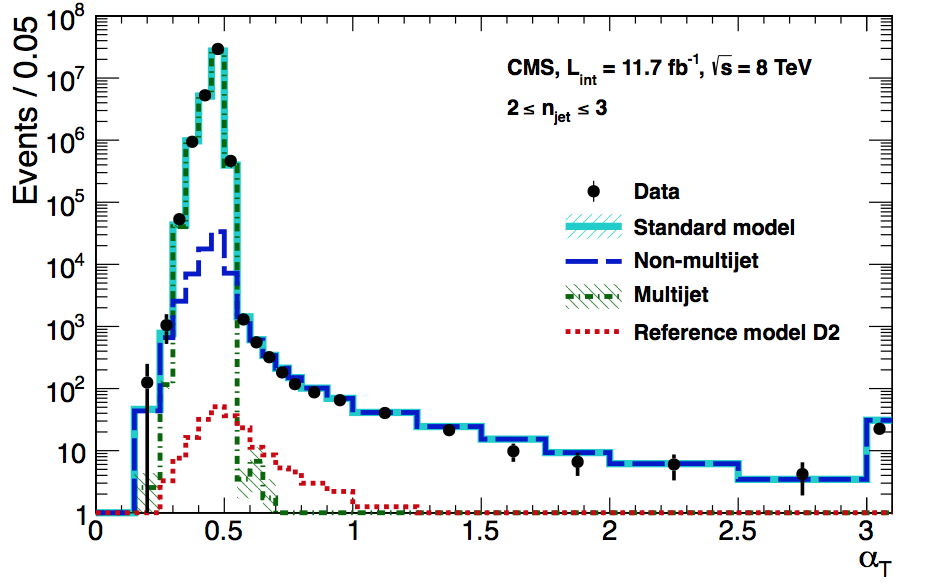
\includegraphics[width=0.8\linewidth]{alphaT1_bkgd}
	\end{center}
	\caption{The $\alpha_T$ values for events with $H_T>375$ GeV and 2 to 3 jets that pass all other cuts imposed in the $\alpha_T$ analysis. The green dotted line shows the expected multijet QCD background that can be removed with an appropriate cut on $\alpha_T$ \cite{AlphaT8TeVChatrchyan:2013lya}}
	\label{fig:alphaT}
\end{figure}

\subsection{The \boldmath $\alpha_T$ analysis}

The only genuine source of missing transverse energy ($\cancel{E}_T$) in the SM is electroweak neutrino production. In these cases an associated lepton is simultaneously produced. This background is minimised by vetoing any events with isolated \footnote{A particle is isolated if the energy of other particles within a cone of $R\equiv\sqrt{(\Delta\phi)^2+(\Delta\eta)^2}=0.3$, where $\phi$ is the azimuthal angle and $\eta$ the pseudorapidity, do not add up to a significant proportion of the particle's momentum, typically $~10$\%} leptons of $p_T>10$~GeV. To ensure a fully hadronic final state there is also a veto on photons of $p_T>25$~GeV. Further, to reduce the ``lost lepton'' backgrounds from W~+~jets 
and $t\bar{t}$, events containing single isolated tracks with $p_T >10$~GeV and $|\eta| < 2.5$ are vetoed.
\\\\
Events are also required to contain at least one $p_T>100$~GeV and one $p_T>40$~GeV jet, where the jets are well reconstructed in the central region, $|\eta|<3$. If any jets fall outside the $\eta$ range, the event is vetoed. Significant hadronic activity is selected for by requiring $H_T>200$~GeV. Events are categorised based on the number of jets, the number of jets with a reconstructed b-quark and the value of $H_T$. 
\\\\
Due to the reduction in QCD cross section at high values of $H_T$, the $\alpha_T$ cut is reduced with this variable while keeping a consistent effective $\cancel{H_T}$ value, see Table~\ref{tab:alphat-thresholds}. Additional cleaning cuts on the ratio of $\cancel{H_T}/\cancel{E_T}$ are also required to reduce instances of high $\cancel{H_T}$ caused by jets just falling out of acceptance. Full details of the analysis as carried out on Run~1 data can be found at \cite{AlphaT8TeVChatrchyan:2013lya} and \cite{AlphaT_7TeV_PRLChatrchyan:2011zy}, and ongoing developments for Run~2 at \cite{AN-15-004}.
\\\\

\begin{table}[h!]
  \caption{$\alpha_T$ and (effective) $\cancel{H_T}$ thresholds per $H_T$ bin.\label{tab:alphat-thresholds}}
  \centering
  \footnotesize
  \begin{tabular}{ lcccccc }
    \hline
    \hline
    $H_T$     & 200--250   & 250--300   & 300--350  & 350--400  & 400--800 \\ %& $>$900       \\
    \hline                                                                     
    $alpha_T$      & 0.65       & 0.60       & 0.55      & 0.53      & 0.52     \\  %& 0.505         \\
    "Min $\cancel{H_T}$"   & $\sim$128  & $\sim$138  & $\sim$125 & $\sim$133 & $\sim$137 \\  %& $\sim$126 \\
    \hline
    \hline
  \end{tabular}
\end{table}

\noindent For the prediction of backgrounds and measuring of systematic errors, control samples are defined. These have all the cuts used for the signal selection described above, but require the existence of one or two leptons or a photon. These leptons and photons are ignored in the calculation of any analysis variables. Additionally, in the case of the lepton control sample no, $\alpha_T$ requirement is made.

%% $Id: introduction.tex 34630 2013-04-29 22:53:51Z roldeman $

\section{Interpreting the results of SUSY searches at CMS}
\label{sec:susyModels}


% the susy production bit

The LHC is a 27km circumference hadron synchrotron built on the Franco-Swiss border \cite{LHCMachine} near Geneva. It ran from 2010 to 2013 colliding protons at centre-of-mass energies $\sqrt{s}=7$ and $8$ TeV (Run 1), with detectors built around the beam collecting up to $23.3$~fb$^{-1}$ of data. Preparations are currently underway for Run 2 of the LHC at a full operating energy of $\sqrt{s}=13$ to $14$ TeV in 2015. This upgrade will have a maximum instantaneous luminosity of $1.6\times10^{34}$~cm$^{-2}$s$^{-1}$, more than twice the peak of $7.7\times10^{33}$~cm$^{-2}$s$^{-1}$ reached in 2012 \cite{LHCLuminosityIPAC13}. With this increase in energy and luminosity, potential for the discovery of new physics at the energy frontier is high.  
\\\\
\subsection{Supersymmetry production at the LHC}
As the LHC is a hadron collider, the highest cross section SUSY production processes occur via the strong force \cite{SUSYprimerMartin:1997ns} \cite{SUSYxsections_NewAspectsof_pp_collisions}. These processes result in the production of squarks and gluinos, the SUSY particles with colour charge. In all favoured SUSY models, these relatively heavy particles decay within the detector to a weakly interacting LSP, usually a neutralino \cite{SUSYPhe_hadronic_states_Farrar:1978xj}. In collisions at the LHC this will appear as several hard jets with unbalanced momentum (missing energy). 
\\\\
To interpret the results of SUSY searches simplified models are used. These models include a smaller number of SUSY particles than the MSSM, but allow the representation of event topologies in a consistent way \cite{SimplifiedModelsAlves:2011wf} \cite{MathiasSUSYthesis}. A simplified model representation of hadronic SUSY production and decay can be seen in Fig.~\ref{fig:simpdecays}.
\begin{figure}
	\begin{center}
		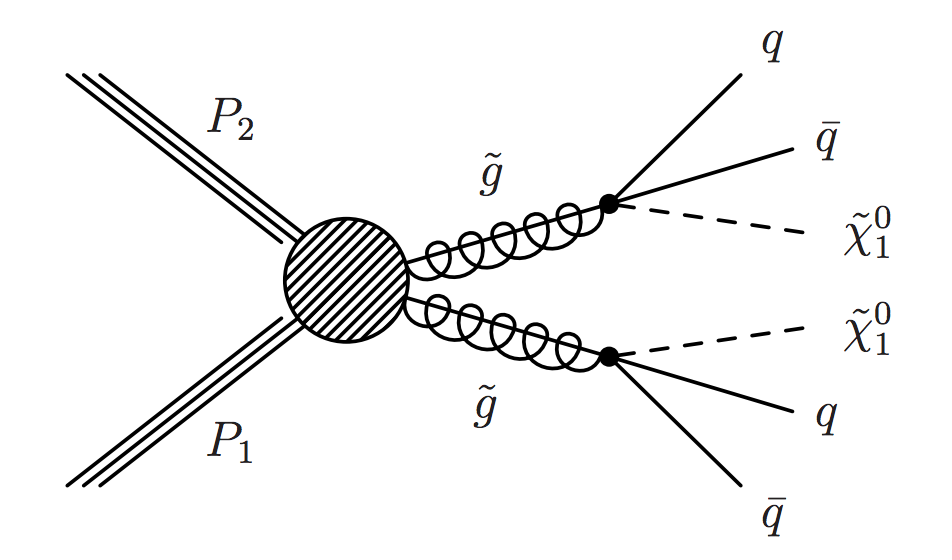
\includegraphics[width=0.4\linewidth]{T1simlifiedpp-gg-qqqqXX}\put(-32,133){(a)}
		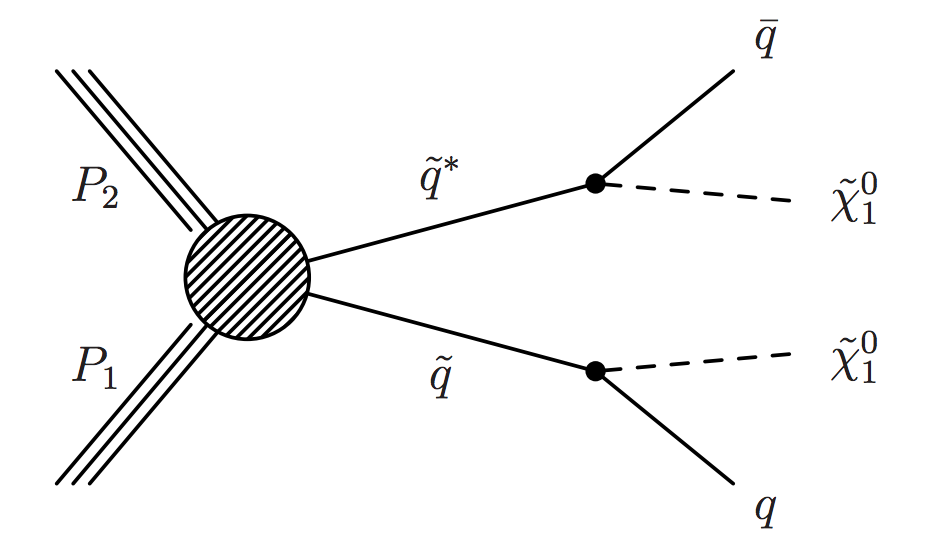
\includegraphics[width=0.4\linewidth]{T2simplifiedpp-qq-qqXX}\put(-32,133){(b)}
	\end{center}
	\caption{Simplified models of SUSY being produced at the LHC and decaying into hadrons plus missing energy \cite{MathiasSUSYthesis}}
	\label{fig:simpdecays}
\end{figure}
\\\\
The $7$ and $8$ TeV run of the LHC has not resulted in any observation of SUSY production as of yet. Instead, limits have been set on the mass of SUSY particles. It is possible that the mass of the SUSY particle has been outside of the energy range of the LHC. With the 2015 upgrade, the cross sections of such supersymmetric particles will increase by at least an order of magnitude, giving a large potential for discovery. It is also possible that the mass splitting of SUSY particles is small, known as compressed spectra. If this is the case the searches at the LHC are not as sensitive, as the energy of the jets produced in the decay to the LSP will be low. This results in a small visible component of missing energy. If SUSY exists at a scale that solves the hierarchy problem with minimal fine tuning, it should be seen at the LHC.






% $Id: introduction.tex 34630 2013-04-29 22:53:51Z roldeman $

\section{The $\alpha_T$ analysis framework}
\label{sec:analysisFw}

To carry out an analysis on the data collected by the CMS detector the physics objects produced in each collision must be reconstructed with software. Each of the collisions are separated into ``events'' based on timing information from the LHC and the pulse shapes of energy deposits within the detector. Algorithms take the inputs from each of the subdetectors per event and use them to reconstruct the different objects produced. A muon, for example, is characterised by a coincidental track in the silicon tracker and hit in the muon chambers. As there are $O(10^6)$ events in a typical dataset, this reconstruction must be carried out reasonably quickly using custom built software.
\\\\
Within the collaboration, subgroups of researchers work to define the individual reconstruction algorithms. This process results in a fixed set of algorithms to be used in the different physics analyses. Carrying out the reconstruction can be computationally expensive, so the predefined reconstruction is carried out centrally, with events grouped into datasets based on their content. In Run~1, a base level of reconstruction was carried out on raw data from CMS to form the ``AOD'' data tier. Analysis groups then carried out their own further reconstruction on the AOD data. Despite the slimming down from the raw data, the AOD tier still has a lot of information unused by many analyses and incomplete reconstruction on many objects to allow for further algorithm customisation. In Run~2 it is proposed to introduce a further data tier ``miniAOD'' that contains less detailed information than the AOD and objects at a more mature stage of reconstruction. This results in data sets that do not require much further processing by the physics analysis groups. The net result is a reduction in the total use of computing time and data storage used by the whole collaboration.
\\\\
To be able to interpret data in the miniAOD format, the $\alpha_T$ analysis framework has been changed significantly. The extra reconstruction and selection required by the analysis have been ported from the old ``ICF'' framework to the ``CMG Tools'' framework, initially developed by the CERN CMS subgroup. The outputs of CMG Tools are very small flat ROOT trees with the base selections in place and only the specific information required by our analysis.
\\\\
With the flat trees produced, it is possible to carry out the high level analysis work flows. These have also been ported to the new ``AlphaTools'' analysis framework and include the systematic error determination through closure tests, accurate estimation of b jet yields in each dataset with the ``b-tag formula method'' \cite{btagformula}, and the statistical interpretation of the results to set limits on or discover particular SUSY processes.

% $Id: introduction.tex 34630 2013-04-29 22:53:51Z roldeman $

\section{Optimising the $\alpha_T$ analysis for Run 2 data}
\label{sec:analysisOptimisation}

The major change with Run~2 of the LHC is the increase in energy to 13~TeV and instantaneous luminosity, to peak at $1.6\times10^{34}$~cm$^{-2}$s$^{-1}$, more than twice the peak of $7.7\times10^{33}$~cm$^{-2}$s$^{-1}$ reached in Run~1 \cite{LHCLuminosityIPAC13}. These two factors result in an increase in the number of simultaneous collisions per event and an increase in cross section for all SM processes. However, for SUSY particles outside the reach of Run~1 analyses, the relative increase in cross section increase should be greater than that for the backgrounds. It is therefore necessary to optimise the analysis to take account of the change in conditions. Some of the optimisations and alterations are discussed in this section, having been studied with $13$~TeV Monte Carlo simulation. The sensitivity to SUSY production is benchmarked using simplified models, each designed to test a particular type of SUSY decay while being model independent~\cite{SimplifiedModelsAlves:2011wf}.
\\\\
Events with a single hard jet and missing energy in their final state are particularly sensitive to the pair production of heavy invisible particles. They usually occur when the invisible system is produced in conjunction with initial or final state radiation from one of the colliding partons. To increase sensitivity to events with this topology, only the lead jet is required to have $p_T>100$~GeV, whereas in the Run~1 analysis this was required of the second leading jet. These extra results are added to an asymmetric jet bin, and have been seen to increase sensitivity to SUSY models with a compressed mass spectrum as well as generic models of dark matter pair production. The increase in yields for a compressed SUSY model by allowing a second jet with $p_T<100$~GeV is evident in Fig.~\ref{fig:asymMotivation}.
\\\\
\begin{figure}[h!]
  \centering
  \subfigure[Second jet $p_T$ for $200$~GeV$<H_T<250$~GeV, $\alpha_T>0.65$]{
    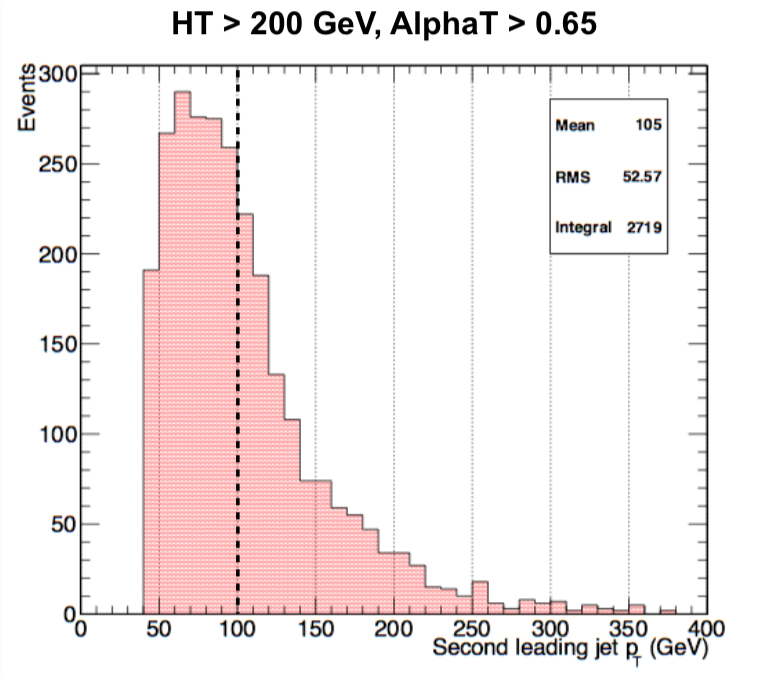
\includegraphics[width=0.5\textwidth]{secondJetPtlowHT}
  }~~
  \subfigure[Second jet $p_T$ for $400$~GeV$<H_T>500$~GeV, $\alpha_T>0.52$]{
    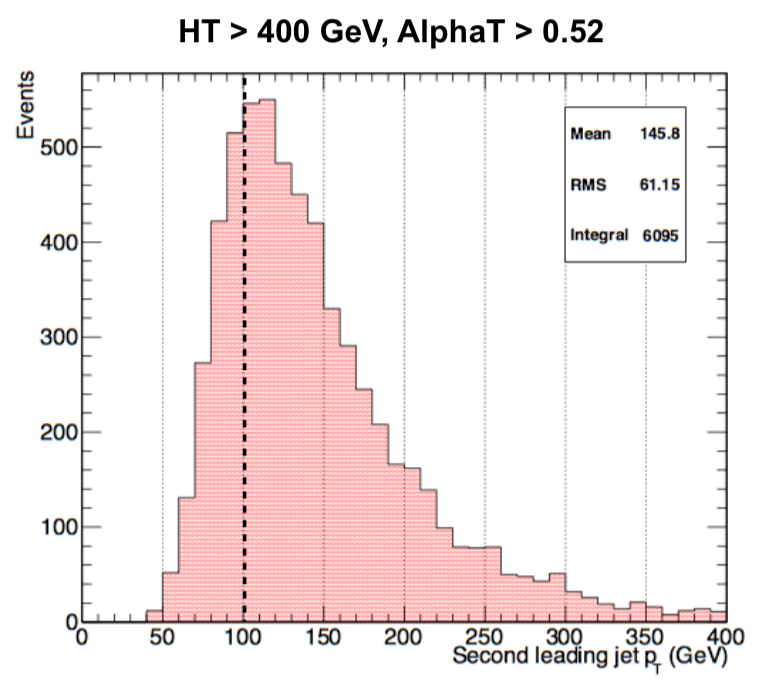
\includegraphics[width=0.5\textwidth]{secondJetPthigherHT}
  }
  \\
  \caption{\label{fig:asymMotivation} The second leading jet $p_T$ for different
  cases of $H_T$ after a baseline signal selection: $N_{jet}\geq2$, lead jet
  $E_T>100\gev$, lepton vetoes. Made with the T2tt ($m_{STOP}=425$~GeV, $m_{LSP}=325$~GeV) simplified model sample.}
\end{figure}

\noindent As the collaboration prepares for Run~2 data taking, the reconstruction algorithms discussed in Sec.~\ref{analysisFw} are developed. As these developments are intended improve overall performance, it is necessary to study the effect of the changes on the $\alpha_T$ analysis and choose the desired parameters for the new algorithms. This also ensures the different analyses in CMS are using consistent object definitions, allowing easy result comparison. The jets we use in the analysis, for example, now utilise tracking information to improve the energy resolution over just the calorimeter information used in Run~1~\cite{ParticleFlow}. Additionally, a new muon reconstruction algorithm improves the efficiency of muon identification but doesn't increase the misidentification rate, allowing a reduction in the W~+~jets and $t\bar{t}$ SM backgrounds. 
\\\\
One additional proposal was a slight change in the lepton isolation algorithm to increase the efficiency of boosted leptons, particularly those produced as the decay products of top quarks. Rather than using a fixed cone around the lepton, the cone size, $R$, was decreased in size according to:
\begin{equation}
R =
  \begin{cases}
    0.2       & p_{T,lep} \leq 50\textrm{GeV}\\
    \frac{10\textrm{GeV}}{p_T,lep}       & 50\textrm{GeV}\geq p_{T,lep} \geq 200\textrm{GeV}\\
    0.05     &  p_{T,lep} \geq 200\textrm{GeV}\\
  \end{cases}
\end{equation}
The result of using this method of isolation on the $\alpha_T$ analysis was checked by running the full analysis with and without the new ``mini isolation'' method. The ratio of the upper limits set on the cross section of a variety of SUSY models can be seen in Table~\ref{tab:miniIsoResult}. In most cases there is an improvement (a decrease in the cross section of the SUSY model that can be excluded). This is most likely due to the improved reduction in $t\bar{t}$ background. However, in the T1tttt model four tops are produced in the final state. By more accurately identifying the leptons in the decay products of these tops, the events move from an apparent hadronic final state to a leptonic one. It is assumed the loss in sensitivity in the $\alpha_T$ analysis will be picked up by a leptonic SUSY analysis.
\\\\
\begin{table}[h!]
  \caption{Changes to sensitivity of various benchmark SUSY models with the new mini isolation algorithm \label{tab:miniIsoResult}}
  \centering
  \footnotesize
  \begin{tabular}{ lcc }
    \hline
    \hline
    SUSY Model     & $\frac{\textrm{mini isolation upper limit on cross section}}{\textrm{normal isolation upper limit on cross section}}$\\ 
    \hline                                                                     
    T1bbbb $m_{\tilde{g}}=1500$~GeV $m_{LSP}=100$~GeV     & 0.95    \\  %& 0.505         \\
    T1tttt $m_{\tilde{g}}=1200$~GeV $m_{LSP}=800$~GeV      & 1.10    \\  %& 0.505         \\
    T2qq $m_{\tilde{t}}=600$~GeV $m_{LSP}=550$~GeV      & 0.97    \\  %& 0.505         \\
    T2tt $m_{\tilde{t}}=500$~GeV $m_{LSP}=325$~GeV       & 0.96    \\  %& 0.505         \\
    \hline
    \hline
  \end{tabular}
\end{table}

\noindent An additional improvement to the analysis is the categorisation of events based on their $\cancel{H_T}$. As SUSY production results in high values of this variable, the signal to background ratio significantly increases at high values of $\cancel{H_T}$. However, the $\alpha_T$ analysis relies on lepton and photon control samples to estimate the SM background in all the analysis bins. This reduces the reliance on the simulation of events with high $\cancel{E_T}$, which isn't well enough understood. There is therefore a limit to how high the bins of $\cancel{H_T}$ can extend, as the control samples must still have some events within these bins. In Run~1 single muon, double muon and single photon control samples were utilised. Single electron and double electron samples, analogous to the muon control samples, are now being introduced to increase the number of events available for background estimation and systematic error determination. Studies on simulation have shown that, with a tight enough requirement on the parameters of the electron identification algorithm, the electron control samples do not suffer from QCD contamination. They therefore effectively double the statistics available in the lepton control samples.


% $Id: introduction.tex 34630 2013-04-29 22:53:51Z roldeman $

\section{The determination of systematic errors in the $\alpha_T$ analysis}
\label{sec:closureTests}







% $Id: introduction.tex 34630 2013-04-29 22:53:51Z roldeman $

\section{Sensitivity to SUSY models with \boldmath $13$~TeV Monte Carlo}
\label{sec:phys14Results}

The projected sensitivity to a variety of benchmark SUSY models was calculated with $13$~TeV MC, testing the full analysis work flow. The models were chosen to have SUSY masses at the edge of the masses excluded in Run~1 with $20/$fb of data. A binned likelihood method was utilised to calculate the $95\%$ Confidence Level (CL) limits on the signal strength. This was carried out for scenarios with $1/$fb and $10/$fb of data. The results are summarised in Table~\ref{tab:results}. In this case, a limit of $1.0$ is equivalent to excluding this model to the $95\%$ CL, greater than $1.0$ means it will not be excluded. With only $1/$fb of data the limits are not very strong, not improving much on the results from Run~1 data \cite{susyRun1Twiki}. However, with $10/$fb, collectable by the end of 2015, there is a good degree of exclusion for most models.
 
\begin{table}[h]
\caption{The expected $95\%$ Confidence Level limits on the signal strength for a variety of benchmark SUSY models. \label{tab:results}}
\centering 
\begin{tabular}{ | l | l | l | }
\hline
	&lumi.=1/fb & lumi.=10/fb  \  \\ \hline
	Model & 95\% CL & 95\% CL \\ \hline
	T2tt $m_{\tilde{t}}=650$ $m_{LSP}=325$ & 3.8 & 1.1 \\ 
	T2tt $m_{\tilde{t}}=500$ $m_{LSP}=325$ & 3.2 & 0.9 \\ 
	T2tt $m_{\tilde{t}}=425$ $m_{LSP}=325$ & 2.3 & 0.7 \\ 
	T2qq $m_{\tilde{t}}=600$ $m_{LSP}=550$ & 0.6 & 0.2 \\ 
	T2qq $m_{\tilde{t}}=1200$ $m_{LSP}=100$ & 2.9 & 0.8 \\ 
	T2bb $m_{\tilde{t}}=900$ $m_{LSP}=100$ & 5.4 & 1.2 \\ 
	T2bb $m_{\tilde{t}}=600$ $m_{LSP}=580$ & 9.3 & 2.6 \\ 
	T1tttt $m_{\tilde{g}}=1500$ $m_{LSP}=100$ & 3.8 & 0.6 \\ 
	T1tttt $m_{\tilde{g}}=1200$ $m_{LSP}=800$ & 4.6 & 1.1 \\ 
	T1qqqq $m_{\tilde{g}}=1400$ $m_{LSP}=800$ & 1.5 & 0.4 \\ 
	T1qqqq $m_{\tilde{g}}=1000$ $m_{LSP}=800$ & 1.0 & 0.3 \\ 
	T1bbbb $m_{\tilde{g}}=1500$ $m_{LSP}=100$ & 1.5 & 0.3 \\ 
	T1bbbb $m_{\tilde{g}}=1000$ $m_{LSP}=900$ & 1.2 & 0.3 \\ \hline
\end{tabular}
\end{table}

\section{Conclusions and further work}
\label{sec:conclusion}

The $\alpha_T$ analysis, investigates an important production channel of electroweak scale SUSY. The preparations of the $\alpha_T$ analysis framework for Run~2 of the LHC is nearing completion. Several analysis optimisations have been carried out, improving the sensitivity of the analysis on bench mark SUSY models. Along with this, the effect of new physics object reconstruction algorithms on the analysis have been investigated. In general a moderate improvement is observed.
\\\\
Further work is required to fully understand the implications of the categorisation of events by $\cancel{H_T}$. The change of the systematic error in this dimension, along with the statistical power of the control samples should be fully determined. The aim always being to ensure the $\alpha_T$ analysis is robust and data driven.
\\\\
With the advent of Run~2 data, the analysis methods and frameworks will be tested and validated. Once enough data has been collected, it will be possible to carry out the full analysis. From the preliminary look with $13$~TeV simulated data, it should be possible to start setting limits on the production of new SUSY processes early into Run~2. This gives a potential for discovery around 2016. 


% Do not include this in analysis note and conference reports
%\section*{Acknowledgements}

\noindent The text below are the acknowledgements as approved by the
collaboration board....


%% $Id: appendix.tex 40350 2013-08-07 13:01:10Z tgershon $
% ===============================================================================
% Purpose: appendix to the standard template: standard symbol alises from Ulrik
% Author: Tomasz Skwarnicki
% Created on: 2009-09-24
% ===============================================================================

\clearpage

{\noindent\bf\Large Appendices}

\appendix

\section{Standard References}
\label{sec:StandardReferences}
Below is a list of common references, as
well as a list of all \lhcb publications. 
As they are already in prepared bib files, they can be used as simply as
\texttt{\textbackslash cite\{Alves:2008zz\}} to get the \lhcb detector paper. 
The references are defined in the files \texttt{main.bib},  \texttt{LHCb-PAPER.bib}, \texttt{LHCb-CONF.bib} and \texttt{LHCb-DP.bib} files, with obvious contents.
Each of these have their {\tt LHCb-ZZZ-20XX-0YY} number as their cite code.
If you believe there is a problem with the formatting or
content of one of the entries, then get in contact with the Editorial
Board rather than just editing it in your local file,
since you are likely to need the latest version just before submiting the article.

\begin{center}
  \begin{tabular}{llc}
\hline
Description & \texttt{cite} code & Reference \\
\hline
\lhcb detector & \texttt{Alves:2008zz} & \cite{Alves:2008zz} \\
%% Trigger & \texttt{LHCb-DP-2012-004} & \cite{LHCb-DP-2012-004} \\
%% RICH & \texttt{LHCb-DP-2012-003} & \cite{LHCb-DP-2012-003} \\
PID performance & \texttt{LHCb-PROC-2011-008} & \cite{LHCb-PROC-2011-008} \\
\lhcb simulation & \texttt{LHCb-PROC-2011-006} & \cite{LHCb-PROC-2011-006} \\
PDG 2012 & \texttt{PDG2012} & \cite{PDG2012} \\
HFAG     & \texttt{HFAG} & \cite{HFAG} \\
\pythia6 & \texttt{Sjostrand:2006za} & \cite{Sjostrand:2006za} \\
\lhcb \pythia tuning & \texttt{LHCb-PROC-2010-056} & \cite{LHCb-PROC-2010-056} \\
\geant & \texttt{Allison:2006ve, *Agostinelli:2002hh} & \cite{Allison:2006ve, *Agostinelli:2002hh} \\
\evtgen & \texttt{Lange:2001uf}  & \cite{Lange:2001uf} \\
\photos & \texttt{Golonka:2005pn}  & \cite{Golonka:2005pn} \\
Crystal Ball function & \texttt{Skwarnicki:1986xj} & \cite{Skwarnicki:1986xj} \\
BDT & \texttt{Breiman} & \cite{Breiman} \\
BDT training & \texttt{AdaBoost} & \cite{AdaBoost} \\
HLT2 topo & \texttt{BBDT} & \cite{BBDT} \\
DecayTreeFitter & \texttt{Hulsbergen:2005pu} & \cite{Hulsbergen:2005pu} \\
\sPlot & \texttt{Pivk:2004ty} & \cite{Pivk:2004ty} \\
Punzi's optimization & \texttt{Punzi:2003bu} & \cite{Punzi:2003bu} \\
\hline
  \end{tabular}
\end{center}

\begin{center}
  %% \caption{\small
  %%   LHCb detector performance papers.
  %% }
  %% \label{tab:LHCb-DPs}
  \begin{tabular}{ll}
    \hline
    \texttt{LHCb-DP} number & Title \\
    \hline
    \texttt{LHCb-DP-2013-001}~\cite{LHCb-DP-2013-001} &
    {\small Performance of the muon identification at LHCb} \\
    \texttt{LHCb-DP-2012-005}~\cite{LHCb-DP-2012-005} &
    {\small Radiation damage in the LHCb Vertex Locator} \\
    \texttt{LHCb-DP-2012-004}~\cite{LHCb-DP-2012-004} &
    {\small The \lhcb trigger and its performance in 2011} \\
    \texttt{LHCb-DP-2012-003}~\cite{LHCb-DP-2012-003} &
    {\small Performance of the \lhcb RICH detector at the LHC} \\
    \texttt{LHCb-DP-2012-002}~\cite{LHCb-DP-2012-002} &
    {\small Performance of the LHCb muon system} \\
    \texttt{LHCb-DP-2012-001}~\cite{LHCb-DP-2012-001} &
    {\small Radiation hardness of the LHCb Outer Tracker} \\
    \texttt{LHCb-DP-2011-002}~\cite{LHCb-DP-2011-002} &
    {\small Simulation of machine induced background ...} \\
    \texttt{LHCb-DP-2011-001}~\cite{LHCb-DP-2011-001} &
    {\small Performance of the LHCb muon system with cosmic rays} \\
    \texttt{LHCb-DP-2010-001}~\cite{LHCb-DP-2010-001} &
    {\small First spatial alignment of the LHCb VELO ...} \\
    \hline
  \end{tabular}
\end{center}

\begin{center}
%  \begin{tabular}{l|l}
\begin{longtable}{ll}
\caption{\small
  LHCb-PAPERs (which have their identifier as their cite code).  
  Note that LHCb-PAPER-2011-039 does not exist.
}
\label{tab:LHCb-PAPERs}
\endfirsthead
\multicolumn{2}{c}{ -- continued from previous page.}
\endhead
\endfoot
\endlastfoot
\hline
\texttt{LHCb-PAPER-2013-054}~\cite{LHCb-PAPER-2013-054} &
\texttt{LHCb-PAPER-2013-053}~\cite{LHCb-PAPER-2013-053} \\
\texttt{LHCb-PAPER-2013-052}~\cite{LHCb-PAPER-2013-052} &
\texttt{LHCb-PAPER-2013-051}~\cite{LHCb-PAPER-2013-051} \\
\texttt{LHCb-PAPER-2013-050}~\cite{LHCb-PAPER-2013-050} &
\texttt{LHCb-PAPER-2013-049}~\cite{LHCb-PAPER-2013-049} \\
\texttt{LHCb-PAPER-2013-048}~\cite{LHCb-PAPER-2013-048} &
\texttt{LHCb-PAPER-2013-047}~\cite{LHCb-PAPER-2013-047} \\
\texttt{LHCb-PAPER-2013-046}~\cite{LHCb-PAPER-2013-046} &
\texttt{LHCb-PAPER-2013-045}~\cite{LHCb-PAPER-2013-045} \\
\texttt{LHCb-PAPER-2013-044}~\cite{LHCb-PAPER-2013-044} &
\texttt{LHCb-PAPER-2013-043}~\cite{LHCb-PAPER-2013-043} \\
\texttt{LHCb-PAPER-2013-042}~\cite{LHCb-PAPER-2013-042} &
\texttt{LHCb-PAPER-2013-041}~\cite{LHCb-PAPER-2013-041} \\
\texttt{LHCb-PAPER-2013-040}~\cite{LHCb-PAPER-2013-040} &
\texttt{LHCb-PAPER-2013-039}~\cite{LHCb-PAPER-2013-039} \\
\texttt{LHCb-PAPER-2013-038}~\cite{LHCb-PAPER-2013-038} &
\texttt{LHCb-PAPER-2013-037}~\cite{LHCb-PAPER-2013-037} \\
\texttt{LHCb-PAPER-2013-036}~\cite{LHCb-PAPER-2013-036} &
\texttt{LHCb-PAPER-2013-035}~\cite{LHCb-PAPER-2013-035} \\
\texttt{LHCb-PAPER-2013-034}~\cite{LHCb-PAPER-2013-034} &
\texttt{LHCb-PAPER-2013-033}~\cite{LHCb-PAPER-2013-033} \\
\texttt{LHCb-PAPER-2013-032}~\cite{LHCb-PAPER-2013-032} &
\texttt{LHCb-PAPER-2013-031}~\cite{LHCb-PAPER-2013-031} \\
\texttt{LHCb-PAPER-2013-030}~\cite{LHCb-PAPER-2013-030} &
\texttt{LHCb-PAPER-2013-029}~\cite{LHCb-PAPER-2013-029} \\
\texttt{LHCb-PAPER-2013-028}~\cite{LHCb-PAPER-2013-028} &
\texttt{LHCb-PAPER-2013-027}~\cite{LHCb-PAPER-2013-027} \\
\texttt{LHCb-PAPER-2013-026}~\cite{LHCb-PAPER-2013-026} &
\texttt{LHCb-PAPER-2013-025}~\cite{LHCb-PAPER-2013-025} \\
\texttt{LHCb-PAPER-2013-024}~\cite{LHCb-PAPER-2013-024} &
\texttt{LHCb-PAPER-2013-023}~\cite{LHCb-PAPER-2013-023} \\
\texttt{LHCb-PAPER-2013-022}~\cite{LHCb-PAPER-2013-022} &
\texttt{LHCb-PAPER-2013-021}~\cite{LHCb-PAPER-2013-021} \\
\texttt{LHCb-PAPER-2013-020}~\cite{LHCb-PAPER-2013-020} &
\texttt{LHCb-PAPER-2013-019}~\cite{LHCb-PAPER-2013-019} \\
\texttt{LHCb-PAPER-2013-018}~\cite{LHCb-PAPER-2013-018} &
\texttt{LHCb-PAPER-2013-017}~\cite{LHCb-PAPER-2013-017} \\
\texttt{LHCb-PAPER-2013-016}~\cite{LHCb-PAPER-2013-016} &
\texttt{LHCb-PAPER-2013-015}~\cite{LHCb-PAPER-2013-015} \\
\texttt{LHCb-PAPER-2013-014}~\cite{LHCb-PAPER-2013-014} &
\texttt{LHCb-PAPER-2013-013}~\cite{LHCb-PAPER-2013-013} \\
\texttt{LHCb-PAPER-2013-012}~\cite{LHCb-PAPER-2013-012} &
\texttt{LHCb-PAPER-2013-011}~\cite{LHCb-PAPER-2013-011} \\
\texttt{LHCb-PAPER-2013-010}~\cite{LHCb-PAPER-2013-010} &
\texttt{LHCb-PAPER-2013-009}~\cite{LHCb-PAPER-2013-009} \\
\texttt{LHCb-PAPER-2013-008}~\cite{LHCb-PAPER-2013-008} &
\texttt{LHCb-PAPER-2013-007}~\cite{LHCb-PAPER-2013-007} \\
\texttt{LHCb-PAPER-2013-006}~\cite{LHCb-PAPER-2013-006} &
\texttt{LHCb-PAPER-2013-005}~\cite{LHCb-PAPER-2013-005} \\
\texttt{LHCb-PAPER-2013-004}~\cite{LHCb-PAPER-2013-004} &
\texttt{LHCb-PAPER-2013-003}~\cite{LHCb-PAPER-2013-003} \\
\texttt{LHCb-PAPER-2013-002}~\cite{LHCb-PAPER-2013-002} &
\texttt{LHCb-PAPER-2013-001}~\cite{LHCb-PAPER-2013-001} \\
\hline
\texttt{LHCb-PAPER-2012-057}~\cite{LHCb-PAPER-2012-057} \\
\texttt{LHCb-PAPER-2012-056}~\cite{LHCb-PAPER-2012-056} & 
\texttt{LHCb-PAPER-2012-055}~\cite{LHCb-PAPER-2012-055} \\
\texttt{LHCb-PAPER-2012-054}~\cite{LHCb-PAPER-2012-054} & 
\texttt{LHCb-PAPER-2012-053}~\cite{LHCb-PAPER-2012-053} \\
\texttt{LHCb-PAPER-2012-052}~\cite{LHCb-PAPER-2012-052} & 
\texttt{LHCb-PAPER-2012-051}~\cite{LHCb-PAPER-2012-051} \\
\texttt{LHCb-PAPER-2012-050}~\cite{LHCb-PAPER-2012-050} & 
\texttt{LHCb-PAPER-2012-049}~\cite{LHCb-PAPER-2012-049} \\
\texttt{LHCb-PAPER-2012-048}~\cite{LHCb-PAPER-2012-048} & 
\texttt{LHCb-PAPER-2012-047}~\cite{LHCb-PAPER-2012-047} \\
\texttt{LHCb-PAPER-2012-046}~\cite{LHCb-PAPER-2012-046} & 
\texttt{LHCb-PAPER-2012-045}~\cite{LHCb-PAPER-2012-045} \\
\texttt{LHCb-PAPER-2012-044}~\cite{LHCb-PAPER-2012-044} & 
\texttt{LHCb-PAPER-2012-043}~\cite{LHCb-PAPER-2012-043} \\
\texttt{LHCb-PAPER-2012-042}~\cite{LHCb-PAPER-2012-042} & 
\texttt{LHCb-PAPER-2012-041}~\cite{LHCb-PAPER-2012-041} \\
\texttt{LHCb-PAPER-2012-040}~\cite{LHCb-PAPER-2012-040} & 
\texttt{LHCb-PAPER-2012-039}~\cite{LHCb-PAPER-2012-039} \\
\texttt{LHCb-PAPER-2012-038}~\cite{LHCb-PAPER-2012-038} & 
\texttt{LHCb-PAPER-2012-037}~\cite{LHCb-PAPER-2012-037} \\
\texttt{LHCb-PAPER-2012-036}~\cite{LHCb-PAPER-2012-036} & 
\texttt{LHCb-PAPER-2012-035}~\cite{LHCb-PAPER-2012-035} \\
\texttt{LHCb-PAPER-2012-034}~\cite{LHCb-PAPER-2012-034} & 
\texttt{LHCb-PAPER-2012-033}~\cite{LHCb-PAPER-2012-033} \\
\texttt{LHCb-PAPER-2012-032}~\cite{LHCb-PAPER-2012-032} & 
\texttt{LHCb-PAPER-2012-031}~\cite{LHCb-PAPER-2012-031} \\
\texttt{LHCb-PAPER-2012-030}~\cite{LHCb-PAPER-2012-030} & 
\texttt{LHCb-PAPER-2012-029}~\cite{LHCb-PAPER-2012-029} \\
\texttt{LHCb-PAPER-2012-028}~\cite{LHCb-PAPER-2012-028} & 
\texttt{LHCb-PAPER-2012-027}~\cite{LHCb-PAPER-2012-027} \\
\texttt{LHCb-PAPER-2012-026}~\cite{LHCb-PAPER-2012-026} & 
\texttt{LHCb-PAPER-2012-025}~\cite{LHCb-PAPER-2012-025} \\
\texttt{LHCb-PAPER-2012-024}~\cite{LHCb-PAPER-2012-024} & 
\texttt{LHCb-PAPER-2012-023}~\cite{LHCb-PAPER-2012-023} \\
\texttt{LHCb-PAPER-2012-022}~\cite{LHCb-PAPER-2012-022} & 
\texttt{LHCb-PAPER-2012-021}~\cite{LHCb-PAPER-2012-021} \\
\texttt{LHCb-PAPER-2012-020}~\cite{LHCb-PAPER-2012-020} & 
\texttt{LHCb-PAPER-2012-019}~\cite{LHCb-PAPER-2012-019} \\
\texttt{LHCb-PAPER-2012-018}~\cite{LHCb-PAPER-2012-018} & 
\texttt{LHCb-PAPER-2012-017}~\cite{LHCb-PAPER-2012-017} \\
\texttt{LHCb-PAPER-2012-016}~\cite{LHCb-PAPER-2012-016} & 
\texttt{LHCb-PAPER-2012-015}~\cite{LHCb-PAPER-2012-015} \\
\texttt{LHCb-PAPER-2012-014}~\cite{LHCb-PAPER-2012-014} & 
\texttt{LHCb-PAPER-2012-013}~\cite{LHCb-PAPER-2012-013} \\
\texttt{LHCb-PAPER-2012-012}~\cite{LHCb-PAPER-2012-012} & 
\texttt{LHCb-PAPER-2012-011}~\cite{LHCb-PAPER-2012-011} \\
\texttt{LHCb-PAPER-2012-010}~\cite{LHCb-PAPER-2012-010} & 
\texttt{LHCb-PAPER-2012-009}~\cite{LHCb-PAPER-2012-009} \\
\texttt{LHCb-PAPER-2012-008}~\cite{LHCb-PAPER-2012-008} & 
\texttt{LHCb-PAPER-2012-007}~\cite{LHCb-PAPER-2012-007} \\
\texttt{LHCb-PAPER-2012-006}~\cite{LHCb-PAPER-2012-006} & 
\texttt{LHCb-PAPER-2012-005}~\cite{LHCb-PAPER-2012-005} \\
\texttt{LHCb-PAPER-2012-004}~\cite{LHCb-PAPER-2012-004} & 
\texttt{LHCb-PAPER-2012-003}~\cite{LHCb-PAPER-2012-003} \\
\texttt{LHCb-PAPER-2012-002}~\cite{LHCb-PAPER-2012-002} & 
\texttt{LHCb-PAPER-2012-001}~\cite{LHCb-PAPER-2012-001} \\
\hline
\texttt{LHCb-PAPER-2011-045}~\cite{LHCb-PAPER-2011-045} & 
\texttt{LHCb-PAPER-2011-044}~\cite{LHCb-PAPER-2011-044} \\
\texttt{LHCb-PAPER-2011-043}~\cite{LHCb-PAPER-2011-043} & 
\texttt{LHCb-PAPER-2011-042}~\cite{LHCb-PAPER-2011-042} \\
\texttt{LHCb-PAPER-2011-041}~\cite{LHCb-PAPER-2011-041} & 
\texttt{LHCb-PAPER-2011-040}~\cite{LHCb-PAPER-2011-040} \\
% \texttt{LHCb-PAPER-2011-039}~\cite{LHCb-PAPER-2011-039} &
\texttt{LHCb-PAPER-2011-038}~\cite{LHCb-PAPER-2011-038} &
\texttt{LHCb-PAPER-2011-037}~\cite{LHCb-PAPER-2011-037} \\
\texttt{LHCb-PAPER-2011-036}~\cite{LHCb-PAPER-2011-036} &
\texttt{LHCb-PAPER-2011-035}~\cite{LHCb-PAPER-2011-035} \\
\texttt{LHCb-PAPER-2011-034}~\cite{LHCb-PAPER-2011-034} &
\texttt{LHCb-PAPER-2011-033}~\cite{LHCb-PAPER-2011-033} \\
\texttt{LHCb-PAPER-2011-032}~\cite{LHCb-PAPER-2011-032} & 
\texttt{LHCb-PAPER-2011-031}~\cite{LHCb-PAPER-2011-031} \\
\texttt{LHCb-PAPER-2011-031}~\cite{LHCb-PAPER-2011-030} &
\texttt{LHCb-PAPER-2011-029}~\cite{LHCb-PAPER-2011-029} \\
\texttt{LHCb-PAPER-2011-028}~\cite{LHCb-PAPER-2011-028} &
\texttt{LHCb-PAPER-2011-027}~\cite{LHCb-PAPER-2011-027} \\
\texttt{LHCb-PAPER-2011-026}~\cite{LHCb-PAPER-2011-026} &
\texttt{LHCb-PAPER-2011-025}~\cite{LHCb-PAPER-2011-025} \\
\texttt{LHCb-PAPER-2011-024}~\cite{LHCb-PAPER-2011-024} &
\texttt{LHCb-PAPER-2011-023}~\cite{LHCb-PAPER-2011-023} \\
\texttt{LHCb-PAPER-2011-023}~\cite{LHCb-PAPER-2011-022} &
\texttt{LHCb-PAPER-2011-021}~\cite{LHCb-PAPER-2011-021} \\
\texttt{LHCb-PAPER-2011-020}~\cite{LHCb-PAPER-2011-020} &
\texttt{LHCb-PAPER-2011-019}~\cite{LHCb-PAPER-2011-019} \\
\texttt{LHCb-PAPER-2011-018}~\cite{LHCb-PAPER-2011-018} &
\texttt{LHCb-PAPER-2011-017}~\cite{LHCb-PAPER-2011-017} \\
\texttt{LHCb-PAPER-2011-016}~\cite{LHCb-PAPER-2011-016} &
\texttt{LHCb-PAPER-2011-015}~\cite{LHCb-PAPER-2011-015} \\
\texttt{LHCb-PAPER-2011-014}~\cite{LHCb-PAPER-2011-014} &
\texttt{LHCb-PAPER-2011-013}~\cite{LHCb-PAPER-2011-013} \\
\texttt{LHCb-PAPER-2011-012}~\cite{LHCb-PAPER-2011-012} &
\texttt{LHCb-PAPER-2011-011}~\cite{LHCb-PAPER-2011-011} \\
\texttt{LHCb-PAPER-2011-010}~\cite{LHCb-PAPER-2011-010} &
\texttt{LHCb-PAPER-2011-009}~\cite{LHCb-PAPER-2011-009} \\
\texttt{LHCb-PAPER-2011-008}~\cite{LHCb-PAPER-2011-008} &
\texttt{LHCb-PAPER-2011-007}~\cite{LHCb-PAPER-2011-007} \\
\texttt{LHCb-PAPER-2011-006}~\cite{LHCb-PAPER-2011-006} &
\texttt{LHCb-PAPER-2011-005}~\cite{LHCb-PAPER-2011-005} \\
\texttt{LHCb-PAPER-2011-004}~\cite{LHCb-PAPER-2011-004} &
\texttt{LHCb-PAPER-2011-003}~\cite{LHCb-PAPER-2011-003} \\
\texttt{LHCb-PAPER-2011-002}~\cite{LHCb-PAPER-2011-002} &
\texttt{LHCb-PAPER-2011-001}~\cite{LHCb-PAPER-2011-001} \\
\hline
\texttt{LHCb-PAPER-2010-002}~\cite{LHCb-PAPER-2010-002} &
\texttt{LHCb-PAPER-2010-001}~\cite{LHCb-PAPER-2010-001} \\
\hline
%  \end{tabular}
\end{longtable}
\end{center}

Some \lhcb papers quoted together will look
like~\cite{LHCb-PAPER-2011-007,LHCb-PAPER-2011-006,
  LHCb-PAPER-2011-005,LHCb-PAPER-2011-004,LHCb-PAPER-2011-003}.
The combination of CMS and LHCb results on $B^0_{(s)} \to \mumu$ should be cited like~\cite{LHCb-CONF-2013-012}.

\section{Standard symbols}

As explained in Sect.~\ref{sec:typography} this appendix contains standard
typesetting of symbols, particle names, units etc.\ in \lhcb
documents. 

In the file \texttt{lhcb-symbols-def.tex}, which is included, a
large number of symbols is defined. While they can lead to quicker
typing, the main reason is to ensure a uniform notation within a
document and between different \lhcb documents. If a symbol
like \texttt{\textbackslash CP} to typeset \CP violation is available
for a unit, particle name, process or whatever, it should be used.  If
you do not agree with the notation you should ask to get the
definition in \texttt{lhcb-symbols-def.tex} changed rather than just
ignoring it.

All the main particles have been given symbols. The \B mesons are thus
named \Bp, \Bd, \Bs, and \Bc. There is no need to go into math mode to
use particle names, thus saving the typing of many \$ signs. By
default particle names are typeset in italic type to agree with the
PDG preference. To get roman particle
names you can just change 
\texttt{\textbackslash setboolean\{uprightparticles\}\{false\}}
to \texttt{true} at the top of this template.

There is a large number of units typeset that ensures the correct use
of fonts, capitals and spacing. As an example we have
$\mBs=5366.3\pm0.6\mevcc$. Note that \mum is typeset with an upright
$\upmu$, even if the particle names have slanted greek letters.

A set of useful symbols are defined for working groups. More of these
symbols can be included later. As an example in the Rare Decay group
we have several different analyses looking for a measurement of
\Cpeff7 and \Opep7.

% This is an automatically generated appendix to template.tex. 
% When included it will show all the symbols defined in lhcb-symbols-def.tex.
%
% To regenerate with the latest definitions run the script ./listsymbols

\section{List of all symbols}
\label{sec:listofsymbols}
\subsection{Experiments}
\begin{tabular*}{\linewidth}{@{\extracolsep{\fill}}l@{\extracolsep{0.5cm}}l@{\extracolsep{\fill}}l@{\extracolsep{0.5cm}}l@{\extracolsep{\fill}}l@{\extracolsep{0.5cm}}l}
\texttt{\textbackslash lhcb} & \lhcb & \texttt{\textbackslash atlas} & \atlas & \texttt{\textbackslash cms} & \cms \\
\texttt{\textbackslash alice} & \alice & \texttt{\textbackslash babar} & \babar & \texttt{\textbackslash belle} & \belle \\
\texttt{\textbackslash cleo} & \cleo & \texttt{\textbackslash cdf} & \cdf & \texttt{\textbackslash dzero} & \dzero \\
\texttt{\textbackslash aleph} & \aleph & \texttt{\textbackslash delphi} & \delphi & \texttt{\textbackslash opal} & \opal \\
\texttt{\textbackslash lthree} & \lthree & \texttt{\textbackslash sld} & \sld & \texttt{\textbackslash cern} & \cern \\
\texttt{\textbackslash lhc} & \lhc & \texttt{\textbackslash lep} & \lep & \texttt{\textbackslash tevatron} & \tevatron \\
\end{tabular*}

\subsubsection{LHCb sub-detectors and sub-systems}
\begin{tabular*}{\linewidth}{@{\extracolsep{\fill}}l@{\extracolsep{0.5cm}}l@{\extracolsep{\fill}}l@{\extracolsep{0.5cm}}l@{\extracolsep{\fill}}l@{\extracolsep{0.5cm}}l}
\texttt{\textbackslash velo} & \velo & \texttt{\textbackslash rich} & \rich & \texttt{\textbackslash richone} & \richone \\
\texttt{\textbackslash richtwo} & \richtwo & \texttt{\textbackslash ttracker} & \ttracker & \texttt{\textbackslash intr} & \intr \\
\texttt{\textbackslash st} & \st & \texttt{\textbackslash ot} & \ot & \texttt{\textbackslash spd} & \spd \\
\texttt{\textbackslash presh} & \presh & \texttt{\textbackslash ecal} & \ecal & \texttt{\textbackslash hcal} & \hcal \\
\end{tabular*}

\subsection{Particles}
\subsubsection{Leptons}
\begin{tabular*}{\linewidth}{@{\extracolsep{\fill}}l@{\extracolsep{0.5cm}}l@{\extracolsep{\fill}}l@{\extracolsep{0.5cm}}l@{\extracolsep{\fill}}l@{\extracolsep{0.5cm}}l}
\texttt{\textbackslash electron} & \electron & \texttt{\textbackslash en} & \en & \texttt{\textbackslash ep} & \ep \\
\texttt{\textbackslash epm} & \epm & \texttt{\textbackslash epem} & \epem & \texttt{\textbackslash mmu} & \mmu \\
\texttt{\textbackslash mup} & \mup & \texttt{\textbackslash mun} & \mun & \texttt{\textbackslash mumu} & \mumu \\
\texttt{\textbackslash mtau} & \mtau & \texttt{\textbackslash taup} & \taup & \texttt{\textbackslash taum} & \taum \\
\texttt{\textbackslash tautau} & \tautau & \texttt{\textbackslash ellm} & \ellm & \texttt{\textbackslash ellp} & \ellp \\
\texttt{\textbackslash neu} & \neu & \texttt{\textbackslash neub} & \neub & \texttt{\textbackslash neue} & \neue \\
\texttt{\textbackslash neueb} & \neueb & \texttt{\textbackslash neum} & \neum & \texttt{\textbackslash neumb} & \neumb \\
\texttt{\textbackslash neut} & \neut & \texttt{\textbackslash neutb} & \neutb & \texttt{\textbackslash neul} & \neul \\
\texttt{\textbackslash neulb} & \neulb &  \\
\end{tabular*}

\subsubsection{Gauge bosons and scalars}
\begin{tabular*}{\linewidth}{@{\extracolsep{\fill}}l@{\extracolsep{0.5cm}}l@{\extracolsep{\fill}}l@{\extracolsep{0.5cm}}l@{\extracolsep{\fill}}l@{\extracolsep{0.5cm}}l}
\texttt{\textbackslash g} & \g & \texttt{\textbackslash H} & \H & \texttt{\textbackslash Hp} & \Hp \\
\texttt{\textbackslash Hm} & \Hm & \texttt{\textbackslash Hpm} & \Hpm & \texttt{\textbackslash W} & \W \\
\texttt{\textbackslash Wp} & \Wp & \texttt{\textbackslash Wm} & \Wm & \texttt{\textbackslash Wpm} & \Wpm \\
\texttt{\textbackslash Z} & \Z &  \\
\end{tabular*}

\subsubsection{Quarks}
\begin{tabular*}{\linewidth}{@{\extracolsep{\fill}}l@{\extracolsep{0.5cm}}l@{\extracolsep{\fill}}l@{\extracolsep{0.5cm}}l@{\extracolsep{\fill}}l@{\extracolsep{0.5cm}}l}
\texttt{\textbackslash quark} & \quark & \texttt{\textbackslash quarkbar} & \quarkbar & \texttt{\textbackslash qqbar} & \qqbar \\
\texttt{\textbackslash uquark} & \uquark & \texttt{\textbackslash uquarkbar} & \uquarkbar & \texttt{\textbackslash uubar} & \uubar \\
\texttt{\textbackslash dquark} & \dquark & \texttt{\textbackslash dquarkbar} & \dquarkbar & \texttt{\textbackslash ddbar} & \ddbar \\
\texttt{\textbackslash squark} & \squark & \texttt{\textbackslash squarkbar} & \squarkbar & \texttt{\textbackslash ssbar} & \ssbar \\
\texttt{\textbackslash cquark} & \cquark & \texttt{\textbackslash cquarkbar} & \cquarkbar & \texttt{\textbackslash ccbar} & \ccbar \\
\texttt{\textbackslash bquark} & \bquark & \texttt{\textbackslash bquarkbar} & \bquarkbar & \texttt{\textbackslash bbbar} & \bbbar \\
\texttt{\textbackslash tquark} & \tquark & \texttt{\textbackslash tquarkbar} & \tquarkbar & \texttt{\textbackslash ttbar} & \ttbar \\
\end{tabular*}

\subsubsection{Light mesons}
\begin{tabular*}{\linewidth}{@{\extracolsep{\fill}}l@{\extracolsep{0.5cm}}l@{\extracolsep{\fill}}l@{\extracolsep{0.5cm}}l@{\extracolsep{\fill}}l@{\extracolsep{0.5cm}}l}
\texttt{\textbackslash pion} & \pion & \texttt{\textbackslash piz} & \piz & \texttt{\textbackslash pizs} & \pizs \\
\texttt{\textbackslash pip} & \pip & \texttt{\textbackslash pim} & \pim & \texttt{\textbackslash pipm} & \pipm \\
\texttt{\textbackslash pimp} & \pimp & \texttt{\textbackslash kaon} & \kaon & \texttt{\textbackslash Kb} & \Kb \\
\texttt{\textbackslash Kz} & \Kz & \texttt{\textbackslash Kzb} & \Kzb & \texttt{\textbackslash Kp} & \Kp \\
\texttt{\textbackslash Km} & \Km & \texttt{\textbackslash Kpm} & \Kpm & \texttt{\textbackslash Kmp} & \Kmp \\
\texttt{\textbackslash KS} & \KS & \texttt{\textbackslash KL} & \KL & \texttt{\textbackslash Kstarz} & \Kstarz \\
\texttt{\textbackslash Kstarzb} & \Kstarzb & \texttt{\textbackslash Kstar} & \Kstar & \texttt{\textbackslash Kstarb} & \Kstarb \\
\texttt{\textbackslash Kstarp} & \Kstarp & \texttt{\textbackslash Kstarm} & \Kstarm & \texttt{\textbackslash Kstarpm} & \Kstarpm \\
\texttt{\textbackslash Kstarmp} & \Kstarmp & \texttt{\textbackslash etapr} & \etapr &  \\
\end{tabular*}

\subsubsection{Heavy mesons}
\begin{tabular*}{\linewidth}{@{\extracolsep{\fill}}l@{\extracolsep{0.5cm}}l@{\extracolsep{\fill}}l@{\extracolsep{0.5cm}}l@{\extracolsep{\fill}}l@{\extracolsep{0.5cm}}l}
\texttt{\textbackslash D} & \D & \texttt{\textbackslash Db} & \Db & \texttt{\textbackslash Dz} & \Dz \\
\texttt{\textbackslash Dzb} & \Dzb & \texttt{\textbackslash Dp} & \Dp & \texttt{\textbackslash Dm} & \Dm \\
\texttt{\textbackslash Dpm} & \Dpm & \texttt{\textbackslash Dmp} & \Dmp & \texttt{\textbackslash Dstar} & \Dstar \\
\texttt{\textbackslash Dstarb} & \Dstarb & \texttt{\textbackslash Dstarz} & \Dstarz & \texttt{\textbackslash Dstarzb} & \Dstarzb \\
\texttt{\textbackslash Dstarp} & \Dstarp & \texttt{\textbackslash Dstarm} & \Dstarm & \texttt{\textbackslash Dstarpm} & \Dstarpm \\
\texttt{\textbackslash Dstarmp} & \Dstarmp & \texttt{\textbackslash Ds} & \Ds & \texttt{\textbackslash Dsp} & \Dsp \\
\texttt{\textbackslash Dsm} & \Dsm & \texttt{\textbackslash Dspm} & \Dspm & \texttt{\textbackslash Dsmp} & \Dsmp \\
\texttt{\textbackslash Dss} & \Dss & \texttt{\textbackslash Dssp} & \Dssp & \texttt{\textbackslash Dssm} & \Dssm \\
\texttt{\textbackslash Dsspm} & \Dsspm & \texttt{\textbackslash Dssmp} & \Dssmp & \texttt{\textbackslash B} & \B \\
\texttt{\textbackslash Bbar} & \Bbar & \texttt{\textbackslash Bb} & \Bb & \texttt{\textbackslash Bz} & \Bz \\
\texttt{\textbackslash Bzb} & \Bzb & \texttt{\textbackslash Bu} & \Bu & \texttt{\textbackslash Bub} & \Bub \\
\texttt{\textbackslash Bp} & \Bp & \texttt{\textbackslash Bm} & \Bm & \texttt{\textbackslash Bpm} & \Bpm \\
\texttt{\textbackslash Bmp} & \Bmp & \texttt{\textbackslash Bd} & \Bd & \texttt{\textbackslash Bs} & \Bs \\
\texttt{\textbackslash Bsb} & \Bsb & \texttt{\textbackslash Bdb} & \Bdb & \texttt{\textbackslash Bc} & \Bc \\
\texttt{\textbackslash Bcp} & \Bcp & \texttt{\textbackslash Bcm} & \Bcm & \texttt{\textbackslash Bcpm} & \Bcpm \\
\end{tabular*}

\subsubsection{Onia}
\begin{tabular*}{\linewidth}{@{\extracolsep{\fill}}l@{\extracolsep{0.5cm}}l@{\extracolsep{\fill}}l@{\extracolsep{0.5cm}}l@{\extracolsep{\fill}}l@{\extracolsep{0.5cm}}l}
\texttt{\textbackslash jpsi} & \jpsi & \texttt{\textbackslash psitwos} & \psitwos & \texttt{\textbackslash psiprpr} & \psiprpr \\
\texttt{\textbackslash etac} & \etac & \texttt{\textbackslash chiczero} & \chiczero & \texttt{\textbackslash chicone} & \chicone \\
\texttt{\textbackslash chictwo} & \chictwo & \texttt{\textbackslash OneS} & \OneS & \texttt{\textbackslash TwoS} & \TwoS \\
\texttt{\textbackslash ThreeS} & \ThreeS & \texttt{\textbackslash FourS} & \FourS & \texttt{\textbackslash FiveS} & \FiveS \\
\texttt{\textbackslash chic} & \chic &  \\
\end{tabular*}

\subsubsection{Baryons}
\begin{tabular*}{\linewidth}{@{\extracolsep{\fill}}l@{\extracolsep{0.5cm}}l@{\extracolsep{\fill}}l@{\extracolsep{0.5cm}}l@{\extracolsep{\fill}}l@{\extracolsep{0.5cm}}l}
\texttt{\textbackslash proton} & \proton & \texttt{\textbackslash antiproton} & \antiproton & \texttt{\textbackslash neutron} & \neutron \\
\texttt{\textbackslash antineutron} & \antineutron & \texttt{\textbackslash Deltares} & \Deltares & \texttt{\textbackslash Deltaresbar} & \Deltaresbar \\
\texttt{\textbackslash Xires} & \Xires & \texttt{\textbackslash Xiresbar} & \Xiresbar & \texttt{\textbackslash Lz} & \Lz \\
\texttt{\textbackslash Lbar} & \Lbar & \texttt{\textbackslash Lambdares} & \Lambdares & \texttt{\textbackslash Lambdaresbar} & \Lambdaresbar \\
\texttt{\textbackslash Sigmares} & \Sigmares & \texttt{\textbackslash Sigmaresbar} & \Sigmaresbar & \texttt{\textbackslash Omegares} & \Omegares \\
\texttt{\textbackslash Omegaresbar} & \Omegaresbar & \texttt{\textbackslash Lb} & \Lb & \texttt{\textbackslash Lbbar} & \Lbbar \\
\texttt{\textbackslash Lc} & \Lc & \texttt{\textbackslash Lcbar} & \Lcbar &  \\
\end{tabular*}

\subsection{Physics symbols}
\subsubsection{Decays}
\begin{tabular*}{\linewidth}{@{\extracolsep{\fill}}l@{\extracolsep{0.5cm}}l@{\extracolsep{\fill}}l@{\extracolsep{0.5cm}}l@{\extracolsep{\fill}}l@{\extracolsep{0.5cm}}l}
\texttt{\textbackslash BF} & \BF & \texttt{\textbackslash BRvis} & \BRvis & \texttt{\textbackslash BR} & \BR \\
\texttt{\textbackslash decay[2] \textbackslash decay\{\Pa\}\{\Pb \Pc\}} & \decay{\Pa}{\Pb \Pc} & \texttt{\textbackslash ra} & \ra & \texttt{\textbackslash to} & \to \\
\end{tabular*}

\subsubsection{Lifetimes}
\begin{tabular*}{\linewidth}{@{\extracolsep{\fill}}l@{\extracolsep{0.5cm}}l@{\extracolsep{\fill}}l@{\extracolsep{0.5cm}}l@{\extracolsep{\fill}}l@{\extracolsep{0.5cm}}l}
\texttt{\textbackslash tauBs} & \tauBs & \texttt{\textbackslash tauBd} & \tauBd & \texttt{\textbackslash tauBz} & \tauBz \\
\texttt{\textbackslash tauBu} & \tauBu & \texttt{\textbackslash tauDp} & \tauDp & \texttt{\textbackslash tauDz} & \tauDz \\
\texttt{\textbackslash tauL} & \tauL & \texttt{\textbackslash tauH} & \tauH &  \\
\end{tabular*}

\subsubsection{Masses}
\begin{tabular*}{\linewidth}{@{\extracolsep{\fill}}l@{\extracolsep{0.5cm}}l@{\extracolsep{\fill}}l@{\extracolsep{0.5cm}}l@{\extracolsep{\fill}}l@{\extracolsep{0.5cm}}l}
\texttt{\textbackslash mBd} & \mBd & \texttt{\textbackslash mBp} & \mBp & \texttt{\textbackslash mBs} & \mBs \\
\texttt{\textbackslash mBc} & \mBc & \texttt{\textbackslash mLb} & \mLb &  \\
\end{tabular*}

\subsubsection{EW theory, groups}
\begin{tabular*}{\linewidth}{@{\extracolsep{\fill}}l@{\extracolsep{0.5cm}}l@{\extracolsep{\fill}}l@{\extracolsep{0.5cm}}l@{\extracolsep{\fill}}l@{\extracolsep{0.5cm}}l}
\texttt{\textbackslash grpsuthree} & \grpsuthree & \texttt{\textbackslash grpsutw} & \grpsutw & \texttt{\textbackslash grpuone} & \grpuone \\
\texttt{\textbackslash ssqtw} & \ssqtw & \texttt{\textbackslash csqtw} & \csqtw & \texttt{\textbackslash stw} & \stw \\
\texttt{\textbackslash ctw} & \ctw & \texttt{\textbackslash ssqtwef} & \ssqtwef & \texttt{\textbackslash csqtwef} & \csqtwef \\
\texttt{\textbackslash stwef} & \stwef & \texttt{\textbackslash ctwef} & \ctwef & \texttt{\textbackslash gv} & \gv \\
\texttt{\textbackslash ga} & \ga & \texttt{\textbackslash order} & \order & \texttt{\textbackslash ordalph} & \ordalph \\
\texttt{\textbackslash ordalsq} & \ordalsq & \texttt{\textbackslash ordalcb} & \ordalcb &  \\
\end{tabular*}

\subsubsection{QCD parameters}
\begin{tabular*}{\linewidth}{@{\extracolsep{\fill}}l@{\extracolsep{0.5cm}}l@{\extracolsep{\fill}}l@{\extracolsep{0.5cm}}l@{\extracolsep{\fill}}l@{\extracolsep{0.5cm}}l}
\texttt{\textbackslash as} & \as & \texttt{\textbackslash MSb} & \MSb & \texttt{\textbackslash lqcd} & \lqcd \\
\texttt{\textbackslash qsq} & \qsq &  \\
\end{tabular*}

\subsubsection{CKM, CP violation}
\begin{tabular*}{\linewidth}{@{\extracolsep{\fill}}l@{\extracolsep{0.5cm}}l@{\extracolsep{\fill}}l@{\extracolsep{0.5cm}}l@{\extracolsep{\fill}}l@{\extracolsep{0.5cm}}l}
\texttt{\textbackslash eps} & \eps & \texttt{\textbackslash epsK} & \epsK & \texttt{\textbackslash epsB} & \epsB \\
\texttt{\textbackslash epsp} & \epsp & \texttt{\textbackslash CP} & \CP & \texttt{\textbackslash CPT} & \CPT \\
\texttt{\textbackslash rhobar} & \rhobar & \texttt{\textbackslash etabar} & \etabar & \texttt{\textbackslash Vud} & \Vud \\
\texttt{\textbackslash Vcd} & \Vcd & \texttt{\textbackslash Vtd} & \Vtd & \texttt{\textbackslash Vus} & \Vus \\
\texttt{\textbackslash Vcs} & \Vcs & \texttt{\textbackslash Vts} & \Vts & \texttt{\textbackslash Vub} & \Vub \\
\texttt{\textbackslash Vcb} & \Vcb & \texttt{\textbackslash Vtb} & \Vtb &  \\
\end{tabular*}

\subsubsection{Oscillations}
\begin{tabular*}{\linewidth}{@{\extracolsep{\fill}}l@{\extracolsep{0.5cm}}l@{\extracolsep{\fill}}l@{\extracolsep{0.5cm}}l@{\extracolsep{\fill}}l@{\extracolsep{0.5cm}}l}
\texttt{\textbackslash dm} & \dm & \texttt{\textbackslash dms} & \dms & \texttt{\textbackslash dmd} & \dmd \\
\texttt{\textbackslash DG} & \DG & \texttt{\textbackslash DGs} & \DGs & \texttt{\textbackslash DGd} & \DGd \\
\texttt{\textbackslash Gs} & \Gs & \texttt{\textbackslash Gd} & \Gd & \texttt{\textbackslash MBq} & \MBq \\
\texttt{\textbackslash DGq} & \DGq & \texttt{\textbackslash Gq} & \Gq & \texttt{\textbackslash dmq} & \dmq \\
\texttt{\textbackslash GL} & \GL & \texttt{\textbackslash GH} & \GH & \texttt{\textbackslash DGsGs} & \DGsGs \\
\texttt{\textbackslash Delm} & \Delm & \texttt{\textbackslash ACP} & \ACP & \texttt{\textbackslash Adir} & \Adir \\
\texttt{\textbackslash Amix} & \Amix & \texttt{\textbackslash ADelta} & \ADelta & \texttt{\textbackslash phid} & \phid \\
\texttt{\textbackslash sinphid} & \sinphid & \texttt{\textbackslash phis} & \phis & \texttt{\textbackslash betas} & \betas \\
\texttt{\textbackslash sbetas} & \sbetas & \texttt{\textbackslash stbetas} & \stbetas & \texttt{\textbackslash stphis} & \stphis \\
\texttt{\textbackslash sinphis} & \sinphis &  \\
\end{tabular*}

\subsubsection{Tagging}
\begin{tabular*}{\linewidth}{@{\extracolsep{\fill}}l@{\extracolsep{0.5cm}}l@{\extracolsep{\fill}}l@{\extracolsep{0.5cm}}l@{\extracolsep{\fill}}l@{\extracolsep{0.5cm}}l}
\texttt{\textbackslash edet} & \edet & \texttt{\textbackslash erec} & \erec & \texttt{\textbackslash esel} & \esel \\
\texttt{\textbackslash etrg} & \etrg & \texttt{\textbackslash etot} & \etot & \texttt{\textbackslash mistag} & \mistag \\
\texttt{\textbackslash wcomb} & \wcomb & \texttt{\textbackslash etag} & \etag & \texttt{\textbackslash etagcomb} & \etagcomb \\
\texttt{\textbackslash effeff} & \effeff & \texttt{\textbackslash effeffcomb} & \effeffcomb & \texttt{\textbackslash efftag} & \efftag \\
\texttt{\textbackslash effD} & \effD & \texttt{\textbackslash etagprompt} & \etagprompt & \texttt{\textbackslash etagLL} & \etagLL \\
\end{tabular*}

\subsubsection{Key decay channels}
\begin{tabular*}{\linewidth}{@{\extracolsep{\fill}}l@{\extracolsep{0.5cm}}l@{\extracolsep{\fill}}l@{\extracolsep{0.5cm}}l@{\extracolsep{\fill}}l@{\extracolsep{0.5cm}}l}
\texttt{\textbackslash BdToKstmm} & \BdToKstmm & \texttt{\textbackslash BdbToKstmm} & \BdbToKstmm & \texttt{\textbackslash BsToJPsiPhi} & \BsToJPsiPhi \\
\texttt{\textbackslash BdToJPsiKst} & \BdToJPsiKst & \texttt{\textbackslash BdbToJPsiKst} & \BdbToJPsiKst & \texttt{\textbackslash BsPhiGam} & \BsPhiGam \\
\texttt{\textbackslash BdKstGam} & \BdKstGam & \texttt{\textbackslash BTohh} & \BTohh & \texttt{\textbackslash BdTopipi} & \BdTopipi \\
\texttt{\textbackslash BdToKpi} & \BdToKpi & \texttt{\textbackslash BsToKK} & \BsToKK & \texttt{\textbackslash BsTopiK} & \BsTopiK \\
\end{tabular*}

\subsubsection{Rare decays}
\begin{tabular*}{\linewidth}{@{\extracolsep{\fill}}l@{\extracolsep{0.5cm}}l@{\extracolsep{\fill}}l@{\extracolsep{0.5cm}}l@{\extracolsep{\fill}}l@{\extracolsep{0.5cm}}l}
\texttt{\textbackslash BdKstee} & \BdKstee & \texttt{\textbackslash BdbKstee} & \BdbKstee & \texttt{\textbackslash bsll} & \bsll \\
\texttt{\textbackslash AFB} & \AFB & \texttt{\textbackslash FL} & \FL & \texttt{\textbackslash AT\#1 \textbackslash AT2} & \AT2 \\
\texttt{\textbackslash btosgam} & \btosgam & \texttt{\textbackslash btodgam} & \btodgam & \texttt{\textbackslash Bsmm} & \Bsmm \\
\texttt{\textbackslash Bdmm} & \Bdmm & \texttt{\textbackslash ctl} & \ctl & \texttt{\textbackslash ctk} & \ctk \\
\end{tabular*}

\subsubsection{Wilson coefficients and operators}
\begin{tabular*}{\linewidth}{@{\extracolsep{\fill}}l@{\extracolsep{0.5cm}}l@{\extracolsep{\fill}}l@{\extracolsep{0.5cm}}l@{\extracolsep{\fill}}l@{\extracolsep{0.5cm}}l}
\texttt{\textbackslash C\#1 \textbackslash C9} & \C9 & \texttt{\textbackslash Cp\#1 \textbackslash Cp7} & \Cp7 & \texttt{\textbackslash Ceff\#1 \textbackslash Ceff9  } & \Ceff9   \\
\texttt{\textbackslash Cpeff\#1 \textbackslash Cpeff7} & \Cpeff7 & \texttt{\textbackslash Ope\#1 \textbackslash Ope2} & \Ope2 & \texttt{\textbackslash Opep\#1 \textbackslash Opep7} & \Opep7 \\
\end{tabular*}

\subsubsection{Charm}
\begin{tabular*}{\linewidth}{@{\extracolsep{\fill}}l@{\extracolsep{0.5cm}}l@{\extracolsep{\fill}}l@{\extracolsep{0.5cm}}l@{\extracolsep{\fill}}l@{\extracolsep{0.5cm}}l}
\texttt{\textbackslash xprime} & \xprime & \texttt{\textbackslash yprime} & \yprime & \texttt{\textbackslash ycp} & \ycp \\
\texttt{\textbackslash agamma} & \agamma & \texttt{\textbackslash dkpicf} & \dkpicf &  \\
\end{tabular*}

\subsubsection{QM}
\begin{tabular*}{\linewidth}{@{\extracolsep{\fill}}l@{\extracolsep{0.5cm}}l@{\extracolsep{\fill}}l@{\extracolsep{0.5cm}}l@{\extracolsep{\fill}}l@{\extracolsep{0.5cm}}l}
\texttt{\textbackslash bra[1] \textbackslash bra\{a\}} & \bra{a} & \texttt{\textbackslash ket[1] \textbackslash ket\{b\}} & \ket{b} & \texttt{\textbackslash braket[2] \textbackslash braket\{a\}\{b\}} & \braket{a}{b} \\
\end{tabular*}

\subsection{Units}
\begin{tabular*}{\linewidth}{@{\extracolsep{\fill}}l@{\extracolsep{0.5cm}}l@{\extracolsep{\fill}}l@{\extracolsep{0.5cm}}l@{\extracolsep{\fill}}l@{\extracolsep{0.5cm}}l}
\texttt{\textbackslash unit[1] \textbackslash unit\{kg\}} & \unit{kg} &  \\
\end{tabular*}

\subsubsection{Energy and momentum}
\begin{tabular*}{\linewidth}{@{\extracolsep{\fill}}l@{\extracolsep{0.5cm}}l@{\extracolsep{\fill}}l@{\extracolsep{0.5cm}}l@{\extracolsep{\fill}}l@{\extracolsep{0.5cm}}l}
\texttt{\textbackslash tev} & \tev & \texttt{\textbackslash gev} & \gev & \texttt{\textbackslash mev} & \mev \\
\texttt{\textbackslash kev} & \kev & \texttt{\textbackslash ev} & \ev & \texttt{\textbackslash gevc} & \gevc \\
\texttt{\textbackslash mevc} & \mevc & \texttt{\textbackslash gevcc} & \gevcc & \texttt{\textbackslash gevgevcccc} & \gevgevcccc \\
\texttt{\textbackslash mevcc} & \mevcc &  \\
\end{tabular*}

\subsubsection{Distance and area}
\begin{tabular*}{\linewidth}{@{\extracolsep{\fill}}l@{\extracolsep{0.5cm}}l@{\extracolsep{\fill}}l@{\extracolsep{0.5cm}}l@{\extracolsep{\fill}}l@{\extracolsep{0.5cm}}l}
\texttt{\textbackslash km} & \km & \texttt{\textbackslash m} & \m & \texttt{\textbackslash cm} & \cm \\
\texttt{\textbackslash cma} & \cma & \texttt{\textbackslash mm} & \mm & \texttt{\textbackslash mma} & \mma \\
\texttt{\textbackslash mum} & \mum & \texttt{\textbackslash muma} & \muma & \texttt{\textbackslash nm} & \nm \\
\texttt{\textbackslash fm} & \fm & \texttt{\textbackslash barn} & \barn & \texttt{\textbackslash mbarn} & \mbarn \\
\texttt{\textbackslash mub} & \mub & \texttt{\textbackslash nb} & \nb & \texttt{\textbackslash invnb} & \invnb \\
\texttt{\textbackslash pb} & \pb & \texttt{\textbackslash invpb} & \invpb & \texttt{\textbackslash fb} & \fb \\
\texttt{\textbackslash invfb} & \invfb &  \\
\end{tabular*}

\subsubsection{Time }
\begin{tabular*}{\linewidth}{@{\extracolsep{\fill}}l@{\extracolsep{0.5cm}}l@{\extracolsep{\fill}}l@{\extracolsep{0.5cm}}l@{\extracolsep{\fill}}l@{\extracolsep{0.5cm}}l}
\texttt{\textbackslash sec} & \sec & \texttt{\textbackslash ms} & \ms & \texttt{\textbackslash mus} & \mus \\
\texttt{\textbackslash ns} & \ns & \texttt{\textbackslash ps} & \ps & \texttt{\textbackslash fs} & \fs \\
\texttt{\textbackslash mhz} & \mhz & \texttt{\textbackslash khz} & \khz & \texttt{\textbackslash hz} & \hz \\
\texttt{\textbackslash invps} & \invps & \texttt{\textbackslash yr} & \yr & \texttt{\textbackslash hr} & \hr \\
\end{tabular*}

\subsubsection{Temperature}
\begin{tabular*}{\linewidth}{@{\extracolsep{\fill}}l@{\extracolsep{0.5cm}}l@{\extracolsep{\fill}}l@{\extracolsep{0.5cm}}l@{\extracolsep{\fill}}l@{\extracolsep{0.5cm}}l}
\texttt{\textbackslash degc} & \degc & \texttt{\textbackslash degk} & \degk &  \\
\end{tabular*}

\subsubsection{Material lengths, radiation}
\begin{tabular*}{\linewidth}{@{\extracolsep{\fill}}l@{\extracolsep{0.5cm}}l@{\extracolsep{\fill}}l@{\extracolsep{0.5cm}}l@{\extracolsep{\fill}}l@{\extracolsep{0.5cm}}l}
\texttt{\textbackslash Xrad} & \Xrad & \texttt{\textbackslash NIL} & \NIL & \texttt{\textbackslash mip} & \mip \\
\texttt{\textbackslash neutroneq} & \neutroneq & \texttt{\textbackslash neqcmcm} & \neqcmcm & \texttt{\textbackslash kRad} & \kRad \\
\texttt{\textbackslash MRad} & \MRad & \texttt{\textbackslash ci} & \ci & \texttt{\textbackslash mci} & \mci \\
\end{tabular*}

\subsubsection{Uncertainties}
\begin{tabular*}{\linewidth}{@{\extracolsep{\fill}}l@{\extracolsep{0.5cm}}l@{\extracolsep{\fill}}l@{\extracolsep{0.5cm}}l@{\extracolsep{\fill}}l@{\extracolsep{0.5cm}}l}
\texttt{\textbackslash sx} & \sx & \texttt{\textbackslash sy} & \sy & \texttt{\textbackslash sz} & \sz \\
\texttt{\textbackslash stat} & \stat & \texttt{\textbackslash syst} & \syst &  \\
\end{tabular*}

\subsubsection{Maths}
\begin{tabular*}{\linewidth}{@{\extracolsep{\fill}}l@{\extracolsep{0.5cm}}l@{\extracolsep{\fill}}l@{\extracolsep{0.5cm}}l@{\extracolsep{\fill}}l@{\extracolsep{0.5cm}}l}
\texttt{\textbackslash order} & \order & \texttt{\textbackslash chisq} & \chisq & \texttt{\textbackslash chisqndf} & \chisqndf \\
\texttt{\textbackslash chisqip} & \chisqip & \texttt{\textbackslash chisqvs} & \chisqvs & \texttt{\textbackslash chisqvtx} & \chisqvtx \\
\texttt{\textbackslash deriv} & \deriv & \texttt{\textbackslash gsim} & \gsim & \texttt{\textbackslash lsim} & \lsim \\
\texttt{\textbackslash mean[1] \textbackslash mean\{x\}} & \mean{x} & \texttt{\textbackslash abs[1] \textbackslash abs\{x\}} & \abs{x} & \texttt{\textbackslash Real} & \Real \\
\texttt{\textbackslash Imag} & \Imag & \texttt{\textbackslash PDF} & \PDF & \texttt{\textbackslash sPlot} & \sPlot \\
\texttt{\textbackslash sWeight} & \sWeight &  \\
\end{tabular*}

\subsection{Kinematics}
\subsubsection{Energy, Momenta}
\begin{tabular*}{\linewidth}{@{\extracolsep{\fill}}l@{\extracolsep{0.5cm}}l@{\extracolsep{\fill}}l@{\extracolsep{0.5cm}}l@{\extracolsep{\fill}}l@{\extracolsep{0.5cm}}l}
\texttt{\textbackslash Ebeam} & \Ebeam & \texttt{\textbackslash sqs} & \sqs & \texttt{\textbackslash ptot} & \ptot \\
\texttt{\textbackslash pt} & \pt & \texttt{\textbackslash et} & \et & \texttt{\textbackslash mt} & \mt \\
\texttt{\textbackslash dpp} & \dpp & \texttt{\textbackslash dedx} & \dedx &  \\
\end{tabular*}

\subsubsection{PID}
\begin{tabular*}{\linewidth}{@{\extracolsep{\fill}}l@{\extracolsep{0.5cm}}l@{\extracolsep{\fill}}l@{\extracolsep{0.5cm}}l@{\extracolsep{\fill}}l@{\extracolsep{0.5cm}}l}
\texttt{\textbackslash dllkpi} & \dllkpi & \texttt{\textbackslash dllppi} & \dllppi & \texttt{\textbackslash dllepi} & \dllepi \\
\texttt{\textbackslash dllmupi} & \dllmupi &  \\
\end{tabular*}

\subsubsection{Geometry}
\begin{tabular*}{\linewidth}{@{\extracolsep{\fill}}l@{\extracolsep{0.5cm}}l@{\extracolsep{\fill}}l@{\extracolsep{0.5cm}}l@{\extracolsep{\fill}}l@{\extracolsep{0.5cm}}l}
\texttt{\textbackslash degrees} & \degrees & \texttt{\textbackslash krad} & \krad & \texttt{\textbackslash mrad} & \mrad \\
\texttt{\textbackslash rad} & \rad &  \\
\end{tabular*}

\subsubsection{Accelerator}
\begin{tabular*}{\linewidth}{@{\extracolsep{\fill}}l@{\extracolsep{0.5cm}}l@{\extracolsep{\fill}}l@{\extracolsep{0.5cm}}l@{\extracolsep{\fill}}l@{\extracolsep{0.5cm}}l}
\texttt{\textbackslash betastar} & \betastar & \texttt{\textbackslash lum} & \lum & \texttt{\textbackslash intlum[1] \textbackslash intlum\{2 \,\invfb\}} & \intlum{2 \,\invfb} \\
\end{tabular*}

\subsection{Software}
\subsubsection{Programs}
\begin{tabular*}{\linewidth}{@{\extracolsep{\fill}}l@{\extracolsep{0.5cm}}l@{\extracolsep{\fill}}l@{\extracolsep{0.5cm}}l@{\extracolsep{\fill}}l@{\extracolsep{0.5cm}}l}
\texttt{\textbackslash bcvegpy} & \bcvegpy & \texttt{\textbackslash boole} & \boole & \texttt{\textbackslash brunel} & \brunel \\
\texttt{\textbackslash davinci} & \davinci & \texttt{\textbackslash dirac} & \dirac & \texttt{\textbackslash evtgen} & \evtgen \\
\texttt{\textbackslash fewz} & \fewz & \texttt{\textbackslash fluka} & \fluka & \texttt{\textbackslash ganga} & \ganga \\
\texttt{\textbackslash gaudi} & \gaudi & \texttt{\textbackslash gauss} & \gauss & \texttt{\textbackslash geant} & \geant \\
\texttt{\textbackslash hepmc} & \hepmc & \texttt{\textbackslash herwig} & \herwig & \texttt{\textbackslash moore} & \moore \\
\texttt{\textbackslash neurobayes} & \neurobayes & \texttt{\textbackslash photos} & \photos & \texttt{\textbackslash powheg} & \powheg \\
\texttt{\textbackslash pythia} & \pythia & \texttt{\textbackslash resbos} & \resbos & \texttt{\textbackslash roofit} & \roofit \\
\texttt{\textbackslash root} & \root & \texttt{\textbackslash spice} & \spice & \texttt{\textbackslash urania} & \urania \\
\end{tabular*}

\subsubsection{Languages}
\begin{tabular*}{\linewidth}{@{\extracolsep{\fill}}l@{\extracolsep{0.5cm}}l@{\extracolsep{\fill}}l@{\extracolsep{0.5cm}}l@{\extracolsep{\fill}}l@{\extracolsep{0.5cm}}l}
\texttt{\textbackslash cpp} & \cpp & \texttt{\textbackslash ruby} & \ruby & \texttt{\textbackslash fortran} & \fortran \\
\texttt{\textbackslash svn} & \svn &  \\
\end{tabular*}

\subsubsection{Data processing}
\begin{tabular*}{\linewidth}{@{\extracolsep{\fill}}l@{\extracolsep{0.5cm}}l@{\extracolsep{\fill}}l@{\extracolsep{0.5cm}}l@{\extracolsep{\fill}}l@{\extracolsep{0.5cm}}l}
\texttt{\textbackslash kbytes} & \kbytes & \texttt{\textbackslash kbsps} & \kbsps & \texttt{\textbackslash kbits} & \kbits \\
\texttt{\textbackslash kbsps} & \kbsps & \texttt{\textbackslash mbsps} & \mbsps & \texttt{\textbackslash mbytes} & \mbytes \\
\texttt{\textbackslash mbps} & \mbps & \texttt{\textbackslash mbsps} & \mbsps & \texttt{\textbackslash gbsps} & \gbsps \\
\texttt{\textbackslash gbytes} & \gbytes & \texttt{\textbackslash gbsps} & \gbsps & \texttt{\textbackslash tbytes} & \tbytes \\
\texttt{\textbackslash tbpy} & \tbpy & \texttt{\textbackslash dst} & \dst &  \\
\end{tabular*}

\subsection{Detector related}
\subsubsection{Detector technologies}
\begin{tabular*}{\linewidth}{@{\extracolsep{\fill}}l@{\extracolsep{0.5cm}}l@{\extracolsep{\fill}}l@{\extracolsep{0.5cm}}l@{\extracolsep{\fill}}l@{\extracolsep{0.5cm}}l}
\texttt{\textbackslash nonn} & \nonn & \texttt{\textbackslash ponn} & \ponn & \texttt{\textbackslash nonp} & \nonp \\
\texttt{\textbackslash cvd} & \cvd & \texttt{\textbackslash mwpc} & \mwpc & \texttt{\textbackslash gem} & \gem \\
\end{tabular*}

\subsubsection{Detector components, electronics}
\begin{tabular*}{\linewidth}{@{\extracolsep{\fill}}l@{\extracolsep{0.5cm}}l@{\extracolsep{\fill}}l@{\extracolsep{0.5cm}}l@{\extracolsep{\fill}}l@{\extracolsep{0.5cm}}l}
\texttt{\textbackslash tell1} & \tell1 & \texttt{\textbackslash ukl1} & \ukl1 & \texttt{\textbackslash beetle} & \beetle \\
\texttt{\textbackslash otis} & \otis & \texttt{\textbackslash croc} & \croc & \texttt{\textbackslash carioca} & \carioca \\
\texttt{\textbackslash dialog} & \dialog & \texttt{\textbackslash sync} & \sync & \texttt{\textbackslash cardiac} & \cardiac \\
\texttt{\textbackslash gol} & \gol & \texttt{\textbackslash vcsel} & \vcsel & \texttt{\textbackslash ttc} & \ttc \\
\texttt{\textbackslash ttcrx} & \ttcrx & \texttt{\textbackslash hpd} & \hpd & \texttt{\textbackslash pmt} & \pmt \\
\texttt{\textbackslash specs} & \specs & \texttt{\textbackslash elmb} & \elmb & \texttt{\textbackslash fpga} & \fpga \\
\texttt{\textbackslash plc} & \plc & \texttt{\textbackslash rasnik} & \rasnik & \texttt{\textbackslash elmb} & \elmb \\
\texttt{\textbackslash can} & \can & \texttt{\textbackslash lvds} & \lvds & \texttt{\textbackslash ntc} & \ntc \\
\texttt{\textbackslash adc} & \adc & \texttt{\textbackslash led} & \led & \texttt{\textbackslash ccd} & \ccd \\
\texttt{\textbackslash hv} & \hv & \texttt{\textbackslash lv} & \lv & \texttt{\textbackslash pvss} & \pvss \\
\texttt{\textbackslash cmos} & \cmos & \texttt{\textbackslash fifo} & \fifo & \texttt{\textbackslash ccpc} & \ccpc \\
\end{tabular*}

\subsubsection{Chemical symbols}
\begin{tabular*}{\linewidth}{@{\extracolsep{\fill}}l@{\extracolsep{0.5cm}}l@{\extracolsep{\fill}}l@{\extracolsep{0.5cm}}l@{\extracolsep{\fill}}l@{\extracolsep{0.5cm}}l}
\texttt{\textbackslash cfourften} & \cfourften & \texttt{\textbackslash cffour} & \cffour & \texttt{\textbackslash cotwo} & \cotwo \\
\texttt{\textbackslash csixffouteen} & \csixffouteen & \texttt{\textbackslash mgftwo} & \mgftwo & \texttt{\textbackslash siotwo} & \siotwo \\
\end{tabular*}

\subsection{Special Text }
\begin{tabular*}{\linewidth}{@{\extracolsep{\fill}}l@{\extracolsep{0.5cm}}l@{\extracolsep{\fill}}l@{\extracolsep{0.5cm}}l@{\extracolsep{\fill}}l@{\extracolsep{0.5cm}}l}
\texttt{\textbackslash eg} & \eg & \texttt{\textbackslash ie} & \ie & \texttt{\textbackslash etal} & \etal \\
\texttt{\textbackslash etc} & \etc & \texttt{\textbackslash cf} & \cf & \texttt{\textbackslash ffp} & \ffp \\
\texttt{\textbackslash vs} & \vs &  \\
\end{tabular*}





%Bibtex or Biblatex style
%\addcontentsline{toc}{section}{References}
%\setboolean{inbibliography}{true}
%\bibliographystyle{LHCb}
\printbibliography

\end{document}
